\documentclass[t,xcolor=svgnames]{beamer}
%\documentclass[t,handout,xcolor=svgnames]{beamer}
\usecolortheme[named=DarkOrchid]{structure}
\usepackage{myTheme}
\usepackage[utf8x]{inputenc}
\usepackage[ngerman]{babel}
\beamertemplatetransparentcovered
\beamertemplateplaintoc            % original plain theme adapted for us
%\usepackage{fancyvrb}
\usepackage{listings}
\usepackage{graphicx}
%\usepackage{mybasis}
\usepackage{hyperref}
\hypersetup{urlcolor=DarkOrchid}
\usepackage{pgfpages}
\usepackage{tikz}
\usepackage{graphicx}
<<<<<<< HEAD
<<<<<<< HEAD
\usepackage{gantt}
=======
>>>>>>> Meeting: Presentation for the first expert meeting
=======
\usepackage{gantt}
>>>>>>> Meeting: Gantt

\title[Object-Oriented Language with Subtyping and Subclassing]{$\mathcal{OOPLSS}$}
\subtitle{Bachelor Thesis}
\institute[BFH-TI]{\textbf{Bern University of Applied Sciences}\\
Engineering and Information Technology}
\author[Ruben Bär und Stefan Heinemann]{Ruben Bär und Stefan Heinemann}
<<<<<<< HEAD
<<<<<<< HEAD
\date{31. März 2011}
=======
\date{10. Mai 2010}
>>>>>>> Meeting: Presentation for the first expert meeting
=======
\date{31. März 2011}
>>>>>>> Meeting: Gantt

% New itemize to insert space between items
% 1st param. optional: options for itemize (e.g. <+->)
% 2nd size to add between items
\newenvironment{bigitemize}[2][]%
{\begin{itemize}[#1]\addtolength{\itemsep}{#2}}%
{\end{itemize}}

%
% Package for formatting Listings
%
\renewcommand*\lstlistlistingname{List of Listings}
\definecolor{lbcolor}{rgb}{0.90,0.90,0.90}
\definecolor{commentcolor}{rgb}{0.0,0.80,0.0}
\lstset{ %
	float=h,
  language=Java,
  basicstyle=\footnotesize,
  numbers=left,
  numberstyle=\tiny,
  stepnumber=1,
 % numbersep=5pt,
  backgroundcolor=\color{white},
  showspaces=false,
  showstringspaces=false,
  showtabs=false,
  frame=single,
  tabsize=2,
  captionpos=b,
  breaklines=true,
  breakatwhitespace=false,
  escapeinside={/*}{*/},
	basicstyle=\ttfamily\footnotesize,
	keywordstyle=\color{blue}\bfseries,
	identifierstyle=\color{black},
	commentstyle=\color{commentcolor},
	stringstyle=\color{red}\ttfamily
}

%
% "define" OOPLSS (Based on scala syntax)
%
\lstdefinelanguage{ooplss}{
  morekeywords={abstract,case,catch,class,def,%
    do,else,extends,false,final,finally,%
    for,if,implicit,import,match,mixin,%
    new,null,object,override,package,%
    private,protected,requires,return,sealed,%
    super,this,throw,trait,true,try,self,base,__construct,%
    type,val,var,while,with,yield,MyType,subtypeOf,subclassOf},
  otherkeywords={=>,<-,<\#,<:,>:,\#,@},
  sensitive=true,
  escapeinside={\%}{)},
  morecomment=[l]{//},
  morecomment=[n]{/*}{*/},
  morestring=[b]",
%  morestring=[b]',
  morestring=[b]"""
}

%
% "define" Scala
%
\lstdefinelanguage{scala}{
  morekeywords={abstract,case,catch,class,def,%
    do,else,extends,false,final,finally,%
    for,if,implicit,import,match,mixin,%
    new,null,object,override,package,%
    private,protected,requires,return,sealed,%
    super,this,throw,trait,true,try,self,base,%
    type,val,var,while,with,yield},
  otherkeywords={=>,<-,<\#,<:,>:,@},
  sensitive=true,
  morecomment=[l]{//},
  escapeinside={/*}{*/},
%  morecomment=[n]{/*}{*/},
  morestring=[b]",
%  morestring=[b]',
  morestring=[b]"""
}

\newcommand{\textdef}[1]{\textcolor{DarkOrchid}{\textbf{#1}}}
\newcommand{\textem}[1]{\textcolor{DarkOrchid}{#1}}
\newcommand{\textcode}[1]{\textcolor{DarkOrchid}{\texttt{#1}}}
\newcommand{\ooplss}{\textem{LISA}\xspace}



%\setbeameroption{show notes on second screen} 

\begin{document}
  \mylstset
  
  % $Id: course.tex 245 2008-01-12 15:07:07Z beo1 $

\begin{frame}
  \titlepage
\end{frame}

\begin{frame}[t]{Inhalt}
  \begin{bigitemize}[<+->]{3mm}
    \item<1-> Vorstellen

    \item<2-> $\mathcal{OOPLSS}$

    \item<3-> Zeitplan

    \item<3-> Dokumentation

    \item<4-> Fragen

    \item<5-> Varia und weiteres Vorgehen
  \end{bigitemize}
\end{frame}
                  % outline and organization
<<<<<<< HEAD
<<<<<<< HEAD
<<<<<<< HEAD
  \begin{frame}[t]{Motivation}
  \begin{bigitemize}[<+->]{3mm}
		\item{Neues Gebiet in der Informatik kennenlernen}

		\item{Mischung aus Theorie und Umsetzung}

		\item{Spannende Arbeiten}

		\item{Persönliche Herausforderung}
	\end{bigitemize}
\end{frame}

=======
>>>>>>> Meeting: Gantt
=======
  \begin{frame}[t]{Motivation}
  \begin{bigitemize}[<+->]{3mm}
		\item{Neues Gebiet in der Informatik kennenlernen}

		\item{Mischung aus Theorie und Umsetzung}

		\item{Spannende Arbeiten}

		\item{Persönliche Herausforderung}
	\end{bigitemize}
\end{frame}

>>>>>>> Meeting: Slides written
  %**********************************************************************************
%
% o   o   o   o          Berne University of Applied Sciences
%             :          Engineering and Information Technology
%             :......o   Computer Science Division
%
% ooplss - Type Systems: Theory and Practice
% Ruben Bär
% $Id: ooplss.tex 48 2011-01-21 07:37:36Z barbr2 $
% $Revision: 48 $
%**********************************************************************************
\documentclass{ooplssTemplate}

\usepackage{mathpartir}
\usepackage{color}
\usepackage{listings}
\usepackage{subfigure}
\usepackage{listing}
\usepackage{fancyvrb}
\usepackage{gantt}
\usepackage{lscape}

\lstset{ %
language=Java,                  % choose the language of the code
basicstyle=\footnotesize,       % the size of the fonts that are used for the code
numbers=left,                   % where to put the line-numbers
numberstyle=\footnotesize,      % the size of the fonts that are used for the line-numbers
stepnumber=1,                   % the step between two line-numbers. If it is 1 each line will be numbered
numbersep=5pt,                  % how far the line-numbers are from the code
backgroundcolor=\color{white},  % choose the background color. You must add \usepackage{color}
showspaces=false,               % show spaces adding particular underscores
showstringspaces=false,         % underline spaces within strings
showtabs=false,                 % show tabs within strings adding particular underscores
frame=single,   		            % adds a frame around the code
tabsize=2,  		                % sets default tabsize to 2 spaces
captionpos=b,   		            % sets the caption-position to bottom
breaklines=true,    	          % sets automatic line breaking
breakatwhitespace=false,        % sets if automatic breaks should only happen at whitespace
escapeinside={\%}{)}            % if you want to add a comment within your code
}

%\includeonly{abstract}
% DOCUMENT CONTENT ------------------------------------------------
\begin{document}
\begin{empfile}
\begin{empcmds}
input metauml;
\end{empcmds}

\title{Bachelor Thesis}
\subtitle{Object-Oriented Language with Subtyping and Subclassing}

\author{Ruben Bär\symbolfootnote[1]{\href{mailto:ruben.baer@codedump.ch}{ruben.baer@codedump.ch}}\\
Stefan Heinemann\symbolfootnote[2]{\href{mailto:stefan.heinemann@codedump.ch}{stefan.heinemann@codedump.ch}}}


% Bern University of Applied Sciences - Engineering and Information Technology, Quellgasse 21, 2501 Biel, Switzerland

% project work, 21. february 2011 - 17. june 2011

\maketitle

%**********************************************************************************
%
% o	 o	 o	 o					Berne University of Applied Sciences
%						 :					Engineering and Information Technology
%						 :......o	 Computer Science Division
%
% OOPLSS - Object-Oriented Language with Subtyping and Subclassing
% Bär Ruben, Heinemann Stefan
%**********************************************************************************
\subsection*{Abstract}
Subtyping is a well known type relation in object-oriented
programming languages and is an important aspect of these languages
to support sound type polymorphism. To support type polymorphism,
subtyping has to restrict the subtype declaration to allow safe type
substitutions. This prohibits the specialisation of binary method declarations 
in subtypes. In many popular object-oriented programming languages, the type
hierarchy is implicitly the same as the implementation hierarchy. This
contradicts the notion of inheritance as code reuse and subtyping as type
substitution. To solve this type of problem, parametrisation has been introduced in
different languages which is also known as \emph{generics}. But these do not
tackle recursive types used for binary methods. To solve this problem
the concept of subclassing with a special type variable \mytype has been
introduced which is an implicit type parameter. But languages supporting
the \mytype variable do not allow the programmer to choose the correct
binding of the variable that fits most to the problem under consideration.

Specialising binary methods without bypassing the type system with
unsafe constructs like casts is often not possible since subtyping is
too restrictive even though it is not required for every problem. This
rises the question whether it is possible to introduce a type safe method
for specialising binary methods or not.

This thesis project presents a solution that allows the programmer to
choose the accurate model that fits the problem. This is presented with
the prototypical programming languages \ooplss\footnote{{\bf L}ISA
{\bf I}ncludes {\bf S}ubcl{\bf A}ssing}. To test the assumptions,
an implementation of some of the features was created within this
project. \ooplss supports two kinds of class derivation with different
specialisation semantics. New to subtyping and generics is a proper
subclassing model which supports inheritance.

It could be shown that subclassing and subtyping are not contradicting
models and that they can fit in one language. It avoids complex structures 
for typing binary methods and includes the possibility of safe software 
composition with less restrictions than subtyping.

%What is the problem or question that the work addresses?
%Why is it important?
%How was the investigation undertaken?
%What was found and what does it mean?


%\vfill
%%\subsection*{Zusammenfassung}
%\selectlanguage{ngerman}
%Hier kommt der deutsche Abstract
%
%\selectlanguage{british}
%\vfill


\thispagestyle{empty}

\tableofcontents

\chapter{Introduction}
Only object-oriented programming languages which are statically typed

\section{Purpose and Situation}
\subsection{Motivation}
Broad definition of learning objectives
Context

\subsection{Objectives and Limitations}
research question

Boundaries of this project

\subsection{Preliminary Activities}

\subsection{New Learning Contents}
Specific new content we had to learn for this project.

\section{Related Work}
\cite{bruce_looj:_2004} LOOJ - Eaving LOOM into Java
%\cite{cook_denotational_1989} 
\cite{bracha_mixin-based_1990} Mixin based inheritance \\
\cite{schaerli_traits:_2003} Traits: Composable Units of Behaviour \\
\cite{ducasse_traits:_2006} Traits: A mechanism for fine-grained reuse \\
\cite{cook_inheritance_1990} Inheritance is not Subtyping \\
\cite{taivalsaari_notion_1996} On the notion of inheritance \\
\cite{steffen_higher-order_1994} Higher-Order subtyping \\
\cite{cartwright_compatible_1998} NextGen \\
\cite{malayeri_integrating_2008} Integrating nominal and structural subtyping \\
\cite{bruce_binary_1995} On Binary Methods \\
\cite{gawecki_tool:_1995}  (TooL) -- Integrating subtyping, matching and type quantification \\
\cite{bruce_polytoil:_1995} PolyToil \\
\cite{bruce_subtyping_1997} Subtyping is not a good match for OOL \\
\cite{abadi_subtyping_1996} On Subtyping and Matching \\
\cite{canning_f-bounded_1989} F-Bounded Polymorphism for OOP

\section{Outline of the Document}

%\section{Results}

% estimated pages: 3

\chapter{Project Management and Technologies}
\label{ctr:projectManagement}
\section{Methodologies}
Many different software development processes have risen since the
breakthrough of software developing. Two major trends can be recognised;
Sequential and iterative design processes. Although iterative processes
have many advantages compared to the others, it is difficult to follow
strictly this design method in this context for this project. On one
hand the development time is very short for regular iterations on the
other hand the project includes many non standard design and development
parts where such a process is difficult to perform. For example, extending
subsequently the grammar may end in major changes in a language. However,
a not very strict iterative model is chosen.

\subsection{Implementation Project}
The project aims to show how subclassing and subtyping can be brought
together uniformly. For this a language specification is provided which
is implemented in a prototypical way. Using this implementation and
specification a comparison between \ooplss and Scala will be done to
show where some advantages or drawbacks come with the ideas implemented
in this project thesis.

\subsection{Iterative and Agile Development}
This project was build iteratively in the sense of continuous
refinement in the definition of the language. The language definition and
implementation goes hand in hand and gives direct feedback. This makes it
possible to test the definition on a concrete implementation. Further
parts from extreme programming are used. Mainly the concept of pair
programming for critical parts which provide interfaces between the
compiler stages. Further is a small not every feature proposed implemented.
First of all a core language needs to be fully enrolled which will be refined
step by step.

However, the fact that the project team are not full time students and have
to work beside the study and project work, it is very difficult to plan
reasonable iterations.

\subsection{Test-Driven Development}
A major goal is to provide a good and robust code basis. To ensure that
this claim holds, test-driven development is performed. With the use of
unit tests code breaking changes can be easily detected. This is inevitable
since many parts are highly fragile, e.g., small changes in the grammar can
cause many changes in the code since the grammar will recognise a complete
other language.

\subsection{Regular Meetings}
The Bern University of Applied Science does not provide a major in
topics used in this thesis. To ensure success regular meetings with the
supervisors are hold. With this early divergence and loss of target should
be prevented. A meeting between the students team and the supervisor
should be at least every two weeks.

\section{Project Schedule}
\subsection{Tasks}
\paragraph{Kick-Off}
In this first phase the tasks will be identified and shortly
described. Since the prior knowledge of type systems and programming
languages is needed to understand the task of this project, some
knowledge exchange has to be done. Important papers will get reviewed
and discussed.

\paragraph{Documentation Chapters 2 and 3}
Chapter 2 shows the used project management methodology. It has to be
evaluated how an iterative model can be adopted to be usable in this
subject. Chapter 3 shows the current problems within object-oriented
languages with subtyping and no subclassing. Further the project idea
will get stated along with the benefits that the language will have. Next
to the normal writing work the used tools has to be evaluated

\paragraph{Grammar and Lexer}
Here an abstract syntax is defined. With the chosen parser generator
the lexer part will be defined for the parser work.

\paragraph{Types}
Parallel to the parser the supported type constructs have to be
defined. Detailed type rules are not yet necessary but needed for the
translation definition from the source language to the target language.

\paragraph{Parser}
Based on the used lexer a parser that builds an abstract syntax tree
(AST) needs to be written. Without this tree no further work is possible.

\paragraph{Tree Walker}
For the subsequent tasks a tree walker is inevitable. Without this
neither a symbol table nor a type checker can be built.

\paragraph{Code Translation Definition}
Since the target language does not natively support all the type
constructs used in \ooplss, a strategy needs to be found
how the source code can be translated to the target language to make it
compile there.

\paragraph{Symbol Table Construction}
The symbol table contains the necessary type context information for
type checking the environment under investigation.

\paragraph{Type Checker}
This phase contains two tasks. First the type rules have to be identified
and written down. Consequently, the rules have to be implemented and tested.

\paragraph{Code Translation}
After some type checking the code can be translated to the target language.

\paragraph{Documentation}
All over the project work the documentation will be extended and reflect the work done.

\subsection{Diagram}
\begin{figure}[H]
	\centerline{
		\begin{sideways}
			\begin{gantt}[xunitlength=0.6cm]{12}{17}
	\begin{ganttitle}
		\numtitle{1}{1}{17}{1}
	\end{ganttitle}
	\ganttbar{Kick-Off}{0}{2}
	\ganttbarcon{Documentation Part I / II}{2}{3}
	\ganttbar{Grammar / Lexer}{3}{2}
	\ganttbarcon{Types}{5}{2}
	\ganttbar{Parser}{5}{3} % Con
	\ganttbar{Tree Walking}{8}{1}
	\ganttbarcon{Symbol Table Construction}{9}{1}
	\ganttbar{Type Checker}{9}{6} % Con
	\ganttbar{Code Translation Definition}{6}{2}
	\ganttbarcon{Code Translation}{11}{5}
	\ganttbar{Documentation}{0}{17}

	\ganttcon{5}{3}{5}{5}
	\ganttcon{8}{5}{8}{6}
	\ganttcon{8}{5}{8}{6}
	\ganttcon{9}{6}{9}{8}
\end{gantt}

		\end{sideways}
	}
	\caption{Project flow}
	\label{fig:gantt}
\end{figure}

The Gantt chart in \Cref{fig:gantt} shows the different major parts performed
during the project. This can \emph{not} be understand as a classical Gantt for
sequential design process. It is not intended to show where exactly tasks are
beginning and finishing. However, it shows at which time of the project we had
the major focus of implementation. For example, it is essential to see that some
work will on the parser will be done even during the implementation of the type
checker. This rises the opportunity to add sequential new features to the
language.

\section{Technologies}

\subsection{Tools and Software}
\begin{description}
	\item[ANTLR3] ANTLR\footnote{ANother Tool for Language
	Recognition} is an advanced LL(*) parser generator with support
	for AST\footnote{Abstract Syntax Tree} generation and tree
	walking respectively rewriting.
	\item[ANTLRWork] Workbench for ANTLR grammars with debug
	environment.
	\item[ANTLR IDE] Eclipse plugin for editing ANTLR grammars.
	\item[Apache Ant] Java tool for automated builds.
	\item[Eclipse] Open source integrated development environment
	for Java. Used for writing the non-ANTLR parts.
	\item[Git] Distributed source control system. Used for the
	development and as a replacement for Subversion. The project is
	hosted by \href{https://www.github.com/rubenbaer/ooplss}{GitHub}\footnote{\href{https://www.github.com/rubenbaer/ooplss}{https://www.github.com/rubenbaer/ooplss}}
	\item[GitHub] Free git hosting platform with webinterface. Is
	used for some project management issues. Provides the possibility
	for issue tracking and code reviews.
	\item[GUnit] Unit testing framework for ANTLR grammars.
	\item[Java] Target language of \ooplss and development language
	of the compiler.
	\item[JUnit] Unit testing framework for Java source code.
	\item[\LaTeX] A macro collection for the \TeX system. Used for
	the documentation. Everything is written with \LaTeX.
	\item[Subversion] Source control system with linear history. Used
	in the first weeks.
\end{description}

\subsection{Standards and Guidelines}
The source code of \ooplss, which is written in Java, follows the official
guidelines from Oracle.\footnote{\href{http://www.oracle.com/technetwork/java/codeconv-138413.html}{http://www.oracle.com/technetwork/java/codeconv-138413.html}}

For the project structure an appropriate structure for us was chosen.
A detailed explanation is found in the project root's README
respectively in Listing \ref{lst:README}.

\begin{listing}
	\VerbatimInput[frame=single,numbers=left,firstline=19,lastline=40]{../README.md}
	\caption{Excerpt from README.md}
	\label{lst:README}
\end{listing}

% estimated page count: 10


\part{Theoretical Background}
\chapter{Subtyping vs. Subclassing}
In this chapter we want you to get familiar with the terms subtyping
and subclassing and their differences. Both concepts exist in some of
the widely known object oriented programming languages like Java or C++, but are
usually mixed up.

\section{Sharing types versus implementation}
\label{sec:sharingTypes}

Although the term \emph{class} is used in modern object oriented
languages like Java and C++, the concept behind it is actually the
concept of subtypes.  The word type is in the sense of data type, such
as integer, boolean etc., but could also be extended types like objects
in object oriented languages. They determine the way data is stored and
what operations can be done on them.

In object oriented languages like Java and C++, the type hierarchy
is directly linked to the implementation hierarchy, in other words,
inheritance automatically creates a subtype. Of a theoretical point
of view however, inheritance is merely a mechanism to reuse code in
further specialisations of classes. This leads us to the first conflict:
sharing types vs. the implementation. To understand this have a look at
example \ref{fig:implementationConflict} \cite{simons_theory_2003-4}:
% reference to simons?

\begin{figure}[H]
\center
\begin{emp}[classdiag](20, 20)

Class.Shape("Shapes")()("+move(x, y):Integer", "+drawOn(c: Canvas)");
Class.Ellipse("Ellipse")("f1, f2: Point", "r, s: Integer")();
Class.Rectangle("Rectangle")("o: Point", "w, h: Integer")();
Class.Circle("Circle")("{f1 = f2, r = s}")();
Class.Square("Square")("{w = h}")();

Ellipse.ne = Shape.s + (-10, -20);
Rectangle.nw = Shape.s + (10, -20);
Circle.n = Ellipse.s + (0, -20);
Square.n = Rectangle.s + (0, -20);

drawObjects(Shape, Ellipse, Rectangle, Circle, Square);
link(inheritance)(Ellipse.n -- Shape.s);
link(inheritance)(Rectangle.n -- Shape.s);
link(inheritance)(Circle.n -- Ellipse.s);
link(inheritance)(Square.n -- Rectangle.s);

Class.Point("Point")("x, y: Integer")();

Point.w = Shape.e + (100, 5);
Class.CircleR("Circle")("r: Integer")();
Class.SquareR("Square")("w: Integer")();
Class.EllipseR("Ellipse")("p, q: Integer", "s: Integer")();
Class.RectangleR("Rectangle")("h: Integer")();

CircleR.ne = Point.s + (-10, -20);
EllipseR.n = CircleR.s + (0, -20);
SquareR.nw = Point.s + (10, -20);
RectangleR.n = SquareR.s + (0, -20);

drawObjects(Point, CircleR, SquareR, EllipseR, RectangleR);
link(inheritance)(CircleR.n -- Point.s);
link(inheritance)(EllipseR.n -- CircleR.s);
link(inheritance)(SquareR.n -- Point.s);
link(inheritance)(RectangleR.n -- SquareR.s);

\end{emp}
\caption{Sharing types vs. implementation}
\label{fig:implementationConflict}
\end{figure}

The left hierarchy expresses the conceptual family: A \emph{Circle}
is a special kind of an \emph{Ellipse}, so is \emph{Square} of
a \emph{Rectangle}. These objects do not actually ''extend`` their
parents though, instead, they rather remove properties. For instance, the
\emph{Circle} removes the property of having two radii.  The hierarchy on
the right on the other hand is conceptual nonsense. It shows, however,
how one could want to derive and reuse code, in this case the x and
y coordinates. Because of that, inheritance (and reuse) of code and
subtyping should be treated differently.

\section{Problem of recursive closure}
\label{sec:recursiveClosure}
Another problem of the subtyping concept we nowadays have in most object 
oriented languages is the problem of contravariance: the arguments of a method
that is derived  and overwrites the same method in the super type
can only have a more general or same argument type, but not a more specific one: 

\begin{figure}[H]
\center
\begin{emp}[classdiag](20, 20)

Class.A("A")()("+method(arg: T')");
Class.B("B")()("+method(arg: T)");

B.e = A.w + (-20, 0);
drawObjects(A, B);
link(inheritance)(B.e -- A.w);

\end{emp}
\caption{Contravariance: the argument type in B is more specific than the one in A}
\label{fig:contravariance}
\end{figure}

This restriction makes perfectly sense for the type security in
programming languages. For certain class constellations, it leads to
further problems though.

Assuming there is a class \emph{Animal} that has the method \emph{mate}
that takes an argument of the type \emph{Animal} and returns a type
\emph{Animal}. Intuitively, all other animal types would be derived
from this type, like \emph{Dog} or \emph{Cat} which would have more
specific arguments that accept only values of the type of itself,
so that dogs can only mate with dogs and cats only with cats (figure
\ref{fig:animalContravariance}) \cite{simons_theory_2003-1}. Because of
the contravariance restriction in subtyping this cannot be achieved by
overriding the method with a more specific argument type.

\begin{figure}[H]
\center
\begin{emp}[classdiag](20, 20)

Class.Animal("Animal")()("mate(Animal): Animal");
Class.Dog("Dog")()("mate(Dog): Dog");
Class.Cat("Cat")()("mate(Cat): Cat");

Dog.ne = Animal.s + (-20, -20);
Cat.nw = Animal.s + (20, -20);

drawObjects(Animal, Dog, Cat);
link(inheritance)(Dog.n -- Animal.s);
link(inheritance)(Cat.n -- Animal.s);

\end{emp}
\caption{The arguments are more specific, which is not allowed because of the contravariance rule}
\label{fig:animalContravariance}
\end{figure}

A similar problem arises in the method \emph{Object.equals: Object
$\rightarrow$ Boolean}\footnote{For those not familiar with this
notation: Object.equals: Object $\rightarrow$ Boolean means that
the equals method/function takes an Object and returns a Boolean}
in Java. The class \emph{Object} has an implementation of the equals
method that takes an argument of the type \emph{Object}. All objects
automatically are of the type \emph{Object} in Java.  Because of the
constraint of contravariance, it is not possible to override this method
with a more specific argument type which would be reasonable since it does
not make any sense to compare two objects of different types. Instead,
if the programmer wants to implement a new version of this method, he
has to use instanceof to check whether the given object is of the same
type. A much more elegant solution would be to let the type system of
the programming language do the checking.\\

\section{Schizophrenic self-reference}
\label{sec:schizoReferences}

In objects there has to be some recursion variable that refers to the
object itself, to be able to call methods or use values on self . 
In some languages this is called \emph{self} or \emph{this}, in
this explanation, the term self will be used to refer to this variable. \\

There are two main cases when recursion occurs:
\begin{enumerate}
\item When a method accesses methods or properties of the self object
\item When a method has arguments or return values of the same type as the object
\end{enumerate}

The first case is problematic when objects are derived: it is not quite
clear to which object the self variable should refer after the derivation.
In C++ and Java, the self-reference in inherited methods refers to the
base object that was derived. This means that an object may contain
many versions of self-references, which is called \emph{schizophrenic
self-reference}. Other languages like Smalltalk and Eiffel treat the
self-reference differently: they redirect the self-reference to the
derived object. \\

An example of shizophrenic self-reference could be a two dimensional
vector type \emph{Vec2D} which has two coordinates and the methods
\emph{identity} and \emph{equals}. The identity method returns the
reference to the object itself and the equals method compares two
objects of this type. It therefore takes an argument of the type
\emph{Vec2D}. Assuming there is a subtype \emph{Vec3D} that inherits
all these methods, adds a z coordinate and overrides the equals
method. Let us further assume that the rule of contravariance does not
apply here. Clearly the equals method of \emph{Vec3D} takes an argument
of the type \emph{vec3D}. Listing \ref{fig:schizoListing} shows this
constellation (in pseudo-code):

\begin{figure}[H]
\begin{lstlisting}
class Vec2D {
	int x,y;

	Vec2D identity() {
		return self;
	}

	bool equals(Vec2D vec) {
		return vec.x == self.x && vec.y == self.y;
	}
}

class Vec3D extends Vec2D {
	int z;

	bool equals(Vec2D vec) {
		return vec.x == self.x && vec.y == self.y && vec.z == self.z;
	}
}
\end{lstlisting}
\caption{An example of schizophrenic self-reference}
\label{fig:schizoListing}
\end{figure}

In the derived class \emph{Vec3D} the self reference in the equals 
method refers to a \emph{Vec3D} object while the one in identity
refers to a \emph{Vec2D} object. This is why an instance of the class
\emph{Vec3D} would be schizophrenic.

This is how the fixation of self-references is done in the subtyping
concept: before the combination (i.e. inheritance) of the objects. In the
concept of subclassing however, it is done after the combination.

\section{Subclassing}

The goal of the concept of subclassing is now to provide a somewhat
different kind of inheritance. With this inheritance, the programmer should
be able to inherit code without automatically creating a subtype. 
\marginpar{Mention here that our programming language will support both?}
This solves the problem described in section \ref{sec:sharingTypes}. Since
subclassing does not create subtypes, the restriction of contravariance, 
described in section \ref{sec:recursiveClosure}, is of no relevancy
anymore. And as already mentioned, the fixation of the self
references and types is done after the inheritance, so there will be no
schizophrenic self-references as described in case 1 in 
\ref{sec:schizoReferences}. \\

In subclassing however, the question rises: how should return values
and arguments be typed (see case 2 in \ref{sec:schizoReferences}) when
defining the methods and fields, since the programmer is not able to know
of what type the subclass will be. This is why there has to be some sort
of placeholder for such cases: the \emph{MyType}. The MyType placeholder
is then substituted with the current type after the inheritance.


\chapter{Matching}
% estimated pages: 2-3
Subtyping is one of the most fundamental property in object-oriented languages
in todays ....

\section{Matching as F-Bounded Subtyping}

\section{Matching as Higher-Order Subtyping}



% estimated pages: 7

\chapter{Language Specification}
\label{ctr:languageSpecification}
This chapter contains the language specification of \ooplss.  The first
section defines the fundamental design principles used in further
discussion of the language. Afterwards an overview of the syntax is
given. It needs to be noted that this is just an abstract definition and
differs in some issues from the real syntax implementation which does not
contain left recursion and is specified as LL(2) grammar. This section
is followed by the largest one in this chapter, containing the language
semantics, containing informal as well as formal parts and reflecting
the development of the language and the ideas behind the concepts. A
last section deals with the primitive types.

\section{Design Principles}
\paragraph{Class Based}
Creating new objects is an essential part in object-oriented
programming. \ooplss provides classes as templates for object
creation. The programmer can specify classes of objects and create
instances of them and not directly objects. Classes are considered as
first order constructs. Furthermore a program is a set of classes. Within
classes only methods and data fields are allowed.

\paragraph{Static and Safe Type System}
To reduce the set of type specific runtime exceptions \ooplss is
statically and strongly typed. Every message received by an object will
not end up in a runtime type exception. Nonetheless runtime exceptions
can occur since the type system does not prove that every statement
is possible, e.g., when sending a division by zero message to a number
object, this case, an appropriate exception will be thrown.

\paragraph{Nominal Type System}
\ooplss has a nominal type system for modular type checking. Once the
inheritance relations are checked, it is easy to determine whether
two types are in relation or not. Since \ooplss is translated to Java,
a similar system is used, i.e., a nominal type system is implemented.
It also makes matching as higher-order subtyping tractable.

\paragraph{No Information Hiding}
Since nominal subtyping is used, information hiding has not such an impact
compared to structural subtyping since all fields are automatically
available. This helps to keep the language small.

\paragraph{No Method Overloading}
In the current state of specification \ooplss does not provide a mechanism
for method overloading. Even though this makes some class combinations impossible,
it is less confusing if this case can be omitted.

\paragraph{Single Dispatch}
With the choice of Java as target platform single method dispatch is
implemented, although multiple dispatch would make some translation work
easier and clearer. For a more detailed discussion see \Cref{ctr:discussion}

\section{Syntax}
\subsection{Abstract Syntax}
\label{sec:abstractSyntax}
The abstract syntax gives a short overview of \ooplss. This syntax is
not normalised and does not completely correspond with the syntax used
in the implementation. \\
\begin{listing}
	{\ttfamily\small
	\begin{tabular}[H]{lrll}
		PROG & \lra & CLASSES \\
		CLASSES & \lra & CLASS+ \\
		CLASS & \lra & `class' C$\langle$`['CLASSPPRMS`]'$\rangle$? COMBINERS \\
		& & ~~~~`\{' VARDEF* METHODDEF* CONSTR* `\}' \\
		CLASSPRMS & \lra & CLASSPARAM $\langle$, CLASSPARAM $\rangle$* \\
		CLASSPARAM & \lra & TYPE \\
		 & | & TYPEVAR \match TYPE \\
		COMBINERS & \lra & SUBTYPEOF? SUBCLASSOF? \\
		SUBTYPEOF & \lra & `subtypeOf' TYPE \\
		SUBCLASSOF & \lra & `subclassOf' TYPE $\langle$`,' TYPE $\rangle$* \\
		TYPE & \lra & TYPENAME \\
		& | & TYPEVAR \\
		TYPENAME & \lra & ID \\
		TYPEVAR & \lra & ID \\
		& | & \mytype \\
		VARDEF & \lra & `var' ID `:' TYPE `;' \\
		METHODDEF & \lra & `def' ID `(' PARAMS? `) :' TYPE `\{' EXPR* `\}' \\
		CONSTR & \lra & `def \_\_construct (' PARAMS? `) \{' EXPR* `\}' \\
		EXPR & \lra & VARDEF \\
		& | & BLOCK \\
		& | & ID = EXPR `;' \\
		& | & VARDEF = EXPR `;' \\
		& | & `if (' EXPR `)' EXPR $\langle$ `else' EXPR $\rangle$? \\
		& | & `while (' EXPR `)' EXPR \\
		& | & `new' TYPENAME `(' METHODPARAMS? `)' \\
		& | & EXPR `.' EXPR \\
		& | & EXPR `(' METHODPARAMS? `)' \\
		METHODPARAMS & \lra & EXPR $\langle$ `,' EXPR $\rangle$* \\
		BLOCK & \lra & `\{' EXPR* `\}' \\
		PARAMS & \lra & ID `:' TYPE $\langle$ `,' ID `:' TYPE $\rangle$ \\
		ID & \lra & $\langle$ a-z, A-Z, \_ $\rangle~\langle$ a-z, A-Z, 0-9, \_ $\rangle$*
	\end{tabular}
	}
	\caption{Abstract syntax of \ooplss}
	\label{lst:abstractSyntax}
\end{listing}

\subsection{Names and Identifiers}
Names in \ooplss identify variables, methods, classes and types. The
definition of names can have different origins and depends on the current
context of consideration which is given by its scope.

\subsection{Scopes}
\ooplss uses lexical scoping to define the validity of expressions and
variables which is similar to that of Java. Generally a global
scope exists wherein the class definitions are. Each class entails a class-scope
that contains all fields, including the definition of superclasses and
supertypes. Local scopes exist within methods and can be nested arbitrary.
Nested local scopes can not shadow already bound variables, i.e., definitions
like in Listing \ref{lst:illegalNesting} are not allowed.

\begin{lstlisting}[float=ht,language=ooplss,caption=Variable definition in local scope,label=lst:illegalNesting]
class A {
	var x : B;

	def m(x : C) : Void {
		var x : D; // Illegal variable definition. Shadows local parameter.
	}

	def f() : Void {
		var x : A;
		{
			var x : B; // Illegal variable definition. Shadows local variable.
		}
	}

	def g() : Void {
		{
			var x: A;
		}
		var x : B; // Legal variable definition since x : A is not
							 // valid anymore.
	}
}
\end{lstlisting}
\subsection{Whitespace and Comments}
Whitespace characters and comments separate single tokens in \ooplss. A
whitespace can either be a blank, a tab or a newline character.

Two kinds of comments are possible. First the C-style multi-line comment which
starts with `/*' and ends with `*/'. Everything between these two delimiters
is ignored by the parser. One specialty to note is, that these kind of comments
can not be nested.
The second kind is in the \cpp-style and is a single- line comment which starts
with `//'. The character sequence between this token and the next newline
is ignored.


\section{Language Semantics}
Classes build the foundation of \ooplss with two kinds of combination
mechanisms, \emph{inheritance} and \emph{extending}. The first
one creates a subclass and the second one a subtype of a given
type. For both cases a new keyword is introduced, \emph{subclassOf}
and \emph{subtypeOf}. The difference between them is the moment of
the self-type binding. In formal treatment a class is considered as a
unordered record \cite{simons_theory_2002-1}.

\subsection{Extension as Subtyping}
'Extension` is one sort of class combination in \ooplss. With extension,
the concept of nominal subtyping is implemented which is the same as
\emph{extends} in Java. Since \ooplss knows two sorts of combination operator, a
clearly distinguishable keyword is introduced: \emph{subtypeOf}. Subtyping
can be represented as a record combination operator where the recursive type binding
is performed before the record combination. However, the operator does
not only combine records, it also overrides old fields which are shadowed
by the new record and renames parent fields \cite{simons_theory_2003-2}.

This record extension is semantically equivalent to that of Java. This
makes a straightforward implementation possible and easy to use for
current Java programmers. Listing \ref{lst:subtypeOf} shows an example
of subtyping in \ooplss. Since this is not an important property for the
implementation, this features is abandoned in the concrete implementation.

\begin{lstlisting}[float=ht,language=ooplss,caption=Subtyping in \ooplss,label=lst:subtypeOf]
class A {
	// Defines a method with parameter of type A.
	def m(p : A) : ReturnType { %\ldots) }
}

class B subtypeOf A {
	// Overrides the parent's method m(p) where A' <: A
	def m(p : A') : ReturnType { %\ldots) }
}
\end{lstlisting}

In most of the programming languages exists a keyword \base or
\emph{super} to referencing explicitly a field in the parent class. Since
\ooplss has two derivation operators, it is not possible to give the
keyword a distinct meaning. To access a parent field, the parents type
name can be used as reference to it.

%\subsubsection{Extension Operator}
%An extension operator is a binary operator merging a superclass type operator
%in a new type operator. Informally it is used to combine to classes to a new one
%which combines a class to a record which is a subtype of the original record.
%
%
%\todo{Combination operator (No method overloading)}

\subsection{Inheritance as Subclassing}
Inheritance is the second class object combination operator in
\ooplss. It is postulated by Simons' Theory of Classification
\cite{simons_theory_2004-2}. This combination is not only a sort of class
extension with code reuse where the new class needs to follow subtyping
rules but also avoids the problem of schizophrenic self-reference since
the self-variable binding is performed after the class combination
and follows the notion of inheritance in the classical sense. \ooplss
integrates this second form of combination within the nominal subtyping
model which is used as well. This dual possibility is unseen in current
programming languages.

To represent this kind of class combination the diagrams used in
this documentary differ from classical UML representation. The
dashed lines show a subclass reference between two classes like in
\Cref{fig:subclassCombination}. The solid lines represent the same as
in UML: a subtype relation between two classes.

\begin{figure}
	\centering
	\includedot[scale=0.8]{dot/subclassCombination}
	\caption{Graphical representation of a inheritance class combination}
	\label{fig:subclassCombination}
\end{figure}

Semantically, a subclass is a break in the subtyping hierarchy,
i.e., inheritance combines classes without holding the subsumption
property. This enables \ooplss having a class hierarchy,
whereas in Java completely new classes would be introduced as illustrated
in \Cref{fig:inheritHierarchy}. In Figure \ref{fig:javaHierarchy} the
classes \emph{C'} and \emph{D'} are the classes \C and \D in Figure
\ref{fig:ooplssHierarchy} after the combination and how Java sees the
relation between them.

\begin{figure}
	\centering
	\subfloat[\ooplss hierarchy]{
		\includedot[scale=0.8]{dot/ooplssHierarchy}
		\label{fig:ooplssHierarchy}
	}
	\subfloat[Java hierarchy]{
		\includedot[scale=0.8]{dot/javaHierarchy}
		\label{fig:javaHierarchy}
	}
	\caption{Class relation hierarchy in \ooplss and Java}
	\label{fig:inheritHierarchy}
\end{figure}

Following this semantics the translation of \ooplss-code to
other object-oriented languages can be done as stated in Listing
\ref{lst:subclassOf} and Listing \ref{lst:javaTrans}.

\begin{lstlisting}[float=ht,language=ooplss,caption=Subclassing in \ooplss,label=lst:subclassOf]
class A {
	var a : A;

	def m(o : A) Void {
		m(a); // Recursive call
	}
}

class B subclassOf A {
	def m(o : A) Void {
		m(a);
		A.m(a);
	}
}
\end{lstlisting}

Listing \ref{lst:javaTrans} presents the code that was translated from Listing
\ref{lst:subclassOf} to Java. It demonstrates the clear cut within
the subtyping hierarchy since the whole content of class \A is modified
and copied to class \B.

\begin{lstlisting}[float=ht,caption=Subclassing translated to Java,label=lst:javaTrans]
public class A {
	public A a;

	public void m(A o) {
		m(a); // Recursive call
	}
}

// Subclass of A
public class B {
	public A a;

	private void A$$m(A o) {
		m(a); // Recursion back to original method
	}

	// Override A.m()
	public void m(A o) {
		m(a); // Direct recursion
		A$$m(a); // Recursion call over class A
	}
}
\end{lstlisting}

%\subsubsection{Inheritance Operator}
%\todo{Combination operator}

\subsection{Introducing \mytype}
Subclassing is an other sort of class combination with a
different semantics than class extension. Considering the listings
\ref{lst:subclassOf} and \ref{lst:javaTrans} one may see something rather
strange. While class \A has a recursive object type this is not the case
for class \B. Since these two classes are completely decoupled but the
classes' type is not changed from \A to \B, the expression in Listing
\ref{lst:breakSelf} can not be typed.

\begin{lstlisting}[float=ht,language=ooplss,caption=Illegal method m(o : \A) : \emph{Void} in class \B,label=lst:breakSelf]
class A {
	def m(o : A) : A {
		return m(self); //Works fine in Java
	}
}

class B subclassOf A {
	def m(o : A) : A {
		return m(self); // Breaks in subclass!
	}
}
\end{lstlisting}

This code is illegal because \self is of type \B and subclassing does
not provide subsumption, in other words, \B $\nless$: \A. To overcome this problem,
a special type variable is introduced which is called \mytype.

This type variable is available in every class but has different meanings
depending on the class under consideration. It is the type correspondence
to the \self variable. Definition \ref{def:selfType} reflects this idea.

\begin{defn}[Self Type]
	\label{def:selfType}
	\self : \X and \X <: \mytype
\end{defn}

Listing \ref{lst:fixBreakSelf} fixes the code with the assumption of
definition \ref{def:selfType}.

\begin{lstlisting}[float=ht,language=ooplss,caption=Type safe code with \mytype,label=lst:fixBreakSelf]
class A {
	def m(o : MyType) : MyType {
		return m(self); //Works well
	}
}

class B subclassOf A { three different examples were introduced where subtyping forces the programmer to write code that needs unsafe type casts and runtime checks.
	def m(o : MyType) : MyType {
		MyType A.m(self); // Works fine as well
	}
}
\end{lstlisting}

The demo in Listing \ref{lst:fixBreakSelf} shows how \mytype works
in \ooplss. Semantically this works because every occurrence of \mytype
is replaced with the new type of class \B. In other words, \mytype is
replaced after the classes are combined.

Listing \ref{lst:fixBreakSelf} shows the translation into the corresponding
Java code in \ref{lst:javaTransMyTypeSubclassing}.

The recursive
method calls in method $m(o : MyType)$ makes clear that subclassing
provides a proper possibility for mutual recursion mentioned in
\Cref{sec:schizoReferences}. This behaviour is intended since this gives
programmers the possibility of full control over the recursion
and the correct program flow.

\begin{lstlisting}[float=ht,caption=Subclassing with \mytype translated to Java,label=lst:javaTransMyTypeSubclassing]
public class A {
	public A m(A o) {
		m(this);
	}
}

public class B {
	private B A/*\$\$*/m(B o) {
		return m(this); // Recursion back to original method
	}

	// Override A.m()
	public B m(B o) {
		return A/*\$\$*/m(this); // Recursion call over class A
	}
}
\end{lstlisting}

\subsubsection{\mytype in Subtyping}
\label{ssec:mytypeInSubtype}
The \mytype was introduced to fix typing problems occurring with
inheritance. This raises the question whether a \mytype is suitable
for extension as well. This problem is illustrated in Listing
\ref{lst:myTypeSubtyping}: it is not sure which type the parameter
$o$ should have in class \B, type \B or type \A.

\begin{lstlisting}[float=ht,language=ooplss,caption=\mytype within subtyping contexts,label=lst:myTypeSubtyping]
class A {
	def m(o : MyType) : MyType {
		return m(self);
	}
}

class B subtypeOf A {
	def m(o : MyType) : MyType {
		return A.m(self);
	}
}
\end{lstlisting}

Let us consider the consequences if $o : B$ in class \B. First of all this
method definition would necessarily require that \ooplss would support
method overloading which it does not. But there are other consequences which
are considerably more problematic, such as that $B.m$ would not be a subtype method of the one
provided from class \A. Knowing that $B.m$ is not a subtype of $A.m$
makes it impossible to create mutual recursion which is provided by inheritance
and only naive recursion would be possible within extension. This means
that if method $A.m$ is called there is no possibility to come back to object \B
within this recursion as long as no dynamic dispatch is available since \B can
not provide an own implementation of $m$ with $o : A$. However, even if \B would
provide two implementations of $m$, one with $o : A$ and one with $o : B$, this
would lead to a contradiction if \B is used as a superclass. For this one may
consider \Cref{fig:hierarchy} and its corresponding code in Listing
\ref{lst:mixedHierarchy}. The problem is on line \ref{lst:mixedHierarchy1}.
If this code segment would be combined in class \C, \self would now be of type
\C which is not a subtype of \A.

\begin{figure}[ht]
	\centering
	\includedot[scale=0.8]{dot/fixedSubclassingSubtyping}
	\caption{Subclassing and subtyping hierarchy}
	\label{fig:hierarchy}
\end{figure}

\begin{lstlisting}[float=ht,language=ooplss,caption=Mixed extension and inheritance hierarchy,label=lst:mixedHierarchy]
class A {
	def m(o : MyType) : MyType {
		return m(self);
	}
}

class B subtypeOf A {
	def m(o : MyType) : MyType {
		return A.m(self);
	}

	def m(o : A) : MyType {
		return o.m(self); // Not typeable in class C %\label{lst:mixedHierarchy1})
	}
}

class C subclassOf B {
	def m(o : MyType) : MyType {
		return B.m(self);
	}
}
\end{lstlisting}

For this the self compatibility is defined as follows:

\begin{defn}[Self is compatible with MyType]
	\label{def:selfCompatibility}
	For every class \A it is true that $self : X$ and $X <: MyType$ but not that $A <: MyType$
\end{defn}

\subsubsection{Binding Moment of \mytype}
To fit the behaviour described in \Cref{ssec:mytypeInSubtype} in a
uniform model of extension and inheritance, the moment when the \mytype is
bound to a real type needs to be considered more clearly. Listing
\ref{lst:bindingInMixedHierarchy} shows a mixed class hierarchy in
\ooplss. First of all \B extends \A. Here the \mytype in method $m$ is
not rebound in the subtype class, i.e., the \mytype binding in extension
is performed as early as possible.

This presents the notion of subtyping completely. However, in \B, the \mytype
is not uniformly bound. Method $f$ has another bound of \mytype than
$m$. This works perfectly fine since $B <: A$. Going one step deeper within
the hierarchy, inheritance is performed. In class \C, every occurrence
of \mytype is now rebound to type \C. This works as well since the
\self-type is defined as in definition \ref{def:selfCompatibility}. Now,
\C is also extended in \D where method $g$ is overridden. Here again,
since in extension the binding moment is performed as early as possible,
this fits well into \ooplss' model of class combination.

\begin{lstlisting}[float=ht,language=ooplss,caption=Binding of \self and \mytype in a mixed context,label=lst:bindingInMixedHierarchy]
class A {
	def m(o : MyType) : MyType { // o : A
		return m(self);
	}
}

class B subtypeOf A {
	def m(o : MyType) : MyType { // o : A
		return A.m(self);
	}

	def f(o : MyType) : MyType { // o : B
		return o.f(self);
	}
}

class C subclassOf B { // Rebinds every occurrence of MyType in hierarchy
	def m(o : MyType) : MyType { // o : C
		return B.m(self);
	}

	def g(o : MyType) : MyType { // o : C
		return g(self);
	}
}

class D subtypeOf C {
	def g(o : MyType) : MyType { // o : C
		return g(self);
	}
}
\end{lstlisting}

Although everything is now typeable, the question rises whether this code
provides mutual recursion as desired? Let's consider a method call of $m$
in \C. The method call handle goes correctly to its superclass method
$B.m$. Now here the next problem occurs. Since the base reference
to the supertype is explicit given by the supertype's name, the base call
is passed uniformly to the supertype class which is now a superclass as well.

%
%How is the \base
%reference considered? First of all, a \base reference does not make
%any sense here since \C does not have a supertype except \object and
%\object usually does not provide a method as wanted.

\subsubsection{Resolving Extension Ambiguity}
\label{sec:resolveAmbiguity}
Let's consider the extension and inheritance hierarchy in \Cref{fig:hierarchy}
again. It is clear that \C inherits \B. But what about the extension of \A
with \B? As seen before, inheritance breaks the hierarchy and only
provides a possibility of class combination. This rises the question how the
relation between \A and \B is considered when a subclass of \B exists. If
the self type in \A would be bound before the record combination to
\C, unsafe type constructs could be possible since a
method expecting type \A would not make any sense in class \C. From this
point of view the extension mechanism has two faces: in a pure
subtyping hierarchy it is subtyping and in a subclassing hierarchy the
extension mechanism is inheritance as well.

Knowing this fact, the following type hierarchy in
\Cref{fig:fixedHierarchy} can be generated for the type \C. This makes
it impossible to use an explicit recursive self reference for classes
since they are not subclass compatible anymore, i.e., the \mytype should
be used wherever possible.

\begin{figure}[ht]
	\centering
	\includedot[scale=0.8]{dot/subclassingSubtyping}
	\caption{Subclassing hierarchy for class \C}
	\label{fig:fixedHierarchy}
\end{figure}
%
%\subsubsection{Method Overloading and Mutual Recursion}
%\subsubsection{}

\subsection{Type Relations}
\ooplss knows two different type relations. On one hand subtyping, which
is well known in typed object-oriented programming languages denoted with
<: or as a straight line in diagrams, respectively. On the other hand
there is a matching relation which is used to restrict type parameters
to a given protocol and is denoted with \match or with a dashed line in
diagrams, respectively. \Cref{fig:hierarchy} shows an example of a type
hierarchy in \ooplss.
%Only one subtype relation between type \A
%and \B exists. Between the other types exists a matching relation; \E
%\match \D \match \C \match \A and \E \match \B.

From this and \Cref{sec:resolveAmbiguity} follows directly that these
relations in \Cref{fig:fixedHierarchy} are true:
\begin{align}
B <: A \\
B <\!\!\#~A \label{alg:match} \\
C <\!\!\#~A \\
C <\!\!\#~B
\end{align}

Since \ooplss uses a nominal type system and not a structural one,
matching does only apply on types within the same hierarchy as under
consideration even if other object types would match types of other
hierarchies.

%\subsubsection{Matching Properties}
%\todo{Higher-order subtyping}

\subsubsection{Matching Embeds Subtyping}
Now, after some considerations about matching, let's take a look at
proposition \ref{prop:matching}. Bruce stated that `matching is the
same as subtyping in the absence of the MyType construct.' From this
proposition and definition \ref{def:matchingAsBound} the following theorem
is formulated that subtyping is embedded into matching. That this is true,
follows directly from its definition.

\begin{prop}[Matching embeds subtyping]
	\label{prop:matchinIsSubtyping}
	if $B <: A$ implies $B \mmatch A$
\end{prop}
%
%\begin{proof}
%	For this one may recall how subtyping is to understand.\footnote{See
%	definitions \ref{def:subtypeObject} and \ref{def:methodSubtyping}}.
%
%	Let $B <: A$, $X := \mu \mytype.\{m :
%	B \times \mytype \rightarrow C \} $ and $Y := \mu X. $\todo{Formal Class combiners first needed}

%	\begin{enumerate}
%		\item From definition \ref{def:subtypeObject}
%		follows directly that $Y <: X$.
%
%		\item
%	\end{enumerate}
%\end{proof}

%\subsection{Class Combination Operator Refined}
%\todo{Give a full specification of class combination operator with mytype and base rewriting}

\subsection{Class Parametrisation}
\label{sec:classParametrisation}
So far the introduction of a \mytype and proper inheritance compared to
other languages gives the advantage of proper code reuse within the type
system and specialisation of binary methods. At a first glance all this
seems not very useful since even generics like those from Java do not fit
into this model very well. Furthermore, the matching relation is not used
by method parameters and is not yet introduced into \ooplss.  As seen
in \Cref{ctr:makingSubclassingPractical} matching is used in object
parametrisation and replaces generics, being the theoretical foundation
of Java's or \cs's generics, respectively. These generics does only
allow f-bounds with subtypes but not with subclasses which is different
in \ooplss because of the matching relation between two subclasses.

\subsubsection{Translation by Mimic Templates}
Knowing that \ooplss class parametrisation is not compatible with that
from Java since Java only knows bounds on subtypes, a different more open
solution is needed. Using matching as bound provides information whether
the code within a parametrised class is legal and can be executed on
objects which are within the bound. The type checker ensures that the
code written in \ooplss is type safe and every method call can be
performed without any runtime errors since it is guaranteed that all
used fields are properly available on the passed objects.

Against this background, the \cpp templates might be a good choice for
representing parametric classes.

\begin{quotation}
`A class generated from a class template is a perfectly ordinary
class. Thus, use of a template does not imply any runtime mechanisms
beyond what is used for an equivalent ``hand-written'' class.' -- Bjarne
Stroustrup \cite{stroustrup_c++_2000}
\end{quotation}

Even \cpp templates have different semantics and are not equivalent with
the translation presented here for \ooplss, but the idea is similar,
namely to create specially named classes similar to templates. Listing
\ref{lst:parametrisationOoplss} presents a container class that is
parametrised with a match-bound of \A. Class \B extends class \A and
class \C inherits \A.

Following the definition of matching, both derived classes are not
allowed as parameters of the class \emph{Container} with the type
parameter definition of $T$ \match \A. The use of those classes
is presented in Line \ref{line:useParametrisationOoplss} in Listing
\ref{lst:parametrisationOoplss}. All of these assignments are typeable
and sound since all of these classes provide the methods assumed
by the bound.

\begin{lstlisting}[language=ooplss,caption=Parametrisation in \ooplss,label=lst:parametrisationOoplss]
class Container[T %\match) A] {
	def m(t1 : T, t2 : T) : T {
		t.someAction(t2);
	}
}

class A {
	def someAction(x : MyType) : MyType {
		return self;
	}
}

class B subtypeOf A {
	def someAction(x : MyType) : MyType {
		return self;
	}
}

class C subclassOf A {
	def someAction(x : MyType) : MyType {
		return self;
	}
}

class Main { %\label{line:useParametrisationOoplss})
	def run() : Void {
		var foo : Container[Foo] = new Container[Foo]();
		var bar : Container[Bar] = new Container[Bar]();
		var foobar : Container[FooBar] = new Container[FooBar]();
		foo.m(new Foo());
		bar.m(new Bar());
		foobar.m(new FooBar());
	}
}
\end{lstlisting}

However, Listing \ref{lst:parametrisationJava} shows
how this code is translated to Java and how the idea of templates is
adopted. Similar to \cpp templates, which generates for all distinct
template parameters a new name mangled class, for every parametrised
class a new inner class with is created with name mangling.
These special classes are all sharing the same generic
interface \emph{Container}. The fact that an interface is needed will be
presented in the next section. One may remark that the Java interface
of \emph{Container} has dropped the f-bound. This is necessary since
subclassing would not fulfill the extension boundary in Java.

The Java code that uses the parametrised classes defined in \ooplss is
then done straightforward by replacing the square brackets to dollar
signs as presented in Line \ref{line:useParametrisationJava} of Listing
\ref{lst:parametrisationJava}

\begin{lstlisting}[language=java,caption=Container class translated to Java,label=lst:parametrisationJava]
public interface Container<T> {
	public T m(t T);

	static public class Container$Foo$ implements Container<Foo> {
		public Foo m(t Foo) {
			t.someAction();
		}
	}

	static public class Container$Bar$ implements Container<Bar> {
		public Bar m(t Bar) {
			t.someAction();
		}
	}

	static public class Container$FooBar$ implements Container<FooBar> {
		public FooBar m(t FooBar) {
			t.someAction();
		}
	}
}

public class Main { /*\label{line:useParametrisationJava}*/
	public void run() {
		Container<Foo> foo = new Container.Container$Foo$();
		Container<Bar> bar = new Container.Container$Bar$();
		Container<FooBar> foobar = new Container.Container$FooBar$();
		foo.m(new Foo());
		bar.m(new Bar());
		foobar.m(new FooBar());
	}
}
\end{lstlisting}

\subsubsection{Specialising Parametrised Classes}
As seen in the previous section, parametrising classes with matching
now fits the model well. However, since parametrised classes
can be inherited as well, this will now be presented that this
is straightforward as well. For the sake of simplicity, only the
translated Java code is presented because fields that are not using
parameters are translated in the same manner as in normal classes.
Listing \ref{lst:extendingContainer} shows an extended version of the
\emph{Container} class.

\begin{lstlisting}[language=java,caption=Extending a container class translated to Java,label=lst:extendingContainer]
public interface SpecialContainer<X> extends Container<X> {
	public X f(X x);

	static public class SpecialContainer$Foo$
			extends Container$Foo$
			implements SpecialContainer<Foo> {
		public Foo m(Foo x) {
			return x;
		}
	}

	static public class SpecialContainer$Bar$
			extends Container$Bar$
			implements SpecialContainer<Bar> {
		public Bar m(Bar x) {
			return x;
		}
	}

	static public class SpecialContainer$FooBar$
			extends Container$FooBar$
			implements SpecialContainer<FooBar> {
		public FooBar m(FooBar x) {
			return x;
		}
	}
}
\end{lstlisting}

\subsubsection{Avoid Type Erasure}
The idea of generating new extended classes instead of a runtime generic
support or type erasure is not new even though the idea is a bit different
with the similar consequences.  Cartwright and Steele proposed
another kind of generics in Java competing with GJ\nomenclature{GJ}{The
research language for the Java generics. It is a short form of `Generic
Java'. Due to copyright law, the name is abbreviated} from Odersky and
Wadler and is presented in \cite{cartwright_compatible_1998}. Their
project is called NextGen and is based on Java 1.2. In contrast to GJ
and the current generics implementation in Java, this project provides an
extension that is not backward compatible to non generic code. However,
since no generic types are used at runtime, type parameters are not
erased like in GJ and Java 1.5.

With this, the language gains on runtime expressiveness since an
\emph{instanceof} operator can be introduced to perform checks on type
variables which Java can not, since Java has not runtime type information
after the type erasure is done. Furthermore the creation of new objects
would also be possible as long as a class provides a standard constructor.

As a drawback of creating all these classes, especially  if a language
would support a modular code generation, a more sophisticated bytecode
analysis and engineering is needed, which \ooplss does not have so far.

A further but not so relevant problem is the generated code overhead.

\subsubsection{Implicitly Parametrised Classes with \mytype}
\label{sec:implicitlyMyType}
To conclude this section about parametrisation let's consider the
\mytype construct. As seen in \Cref{ctr:theoreticalBackground}, the
\self variable can be bound to its real type by applying the unbound
type operator recursively. To grasp this notion in \ooplss, classes
can be considered as implicitly parametrised. Since both, subtyping
and subclassing, are available, the type parameter list is extended
with one additional type parameter in every subtype. Only this makes it
possible to derive binary methods in subtypes and subclasses as well. An
explicitly parametrised hypothetical use of \mytype is presented in
Listing \ref{lst:explicitMyType}.

\begin{lstlisting}[language=ooplss,caption=Explicit \mytype parametrisation,label=lst:explicitMyType]
class A[MyType <# A] {
	def m(o : MyType) MyType {
		// Self is explicitly typed in the method.
		return self;
	}
}

class B[MyType <# B, MyType$A$ <# A] subtypeOf A[MyType$A$] {
	// MyType of class A is used in class B
	def m(o : MyType$A$) : MyType$A$ { %\ldots) }
	%\ldots)
}

class C[MyType <# C] subclassOf A[MyType] {
	%\ldots)
}

class D[MyType <# D] subclassOf B[MyType, MyType] {
	%\ldots)
}
\end{lstlisting}

\section{Built-in Types}
\label{sec:builtinTypes}
Within \ooplss exists some built-in types. Even they are represented
as objects they have no methods and can not be derived. They are
similar in use to primitive data types and are defined as such types
to provide simple data types that can be used intuitively. Table
\ref{table:builtinOperations} presents the operators supported by
the types. For an easier treatment of the basic types, the tables
\ref{table:arithmeticOp} - \ref{table:equalityOp} shows the type
compatibilities between two different types using these operators.

To provide simple interaction between \ooplss and the user a \emph{System}
class is introduced that is shipped with every program written in
\ooplss. It has five non-static methods: \textit{print, println,
printlnInt, readln} and \textit{readfile}.

\begin{table}[H]
	\centering
	\begin{tabular}{|>{\bfseries}c|c|c|c|c|c|c|c|c|c|c|} \hline
	& $+$ & $-$ & $*$ & $/$ & $<$ & $>$ & $<=$ & $>=$ & $==$ & $!=$ \\ \hline
	Object & & & & & & & & & $\bullet$ & $\bullet$ \\ \hline
	Int & $\bullet$ & $\bullet$ & $\bullet$ & $\bullet$ & $\bullet$ & $\bullet$ & $\bullet$ & $\bullet$ & $\bullet$ & $\bullet$ \\ \hline
	Float & $\bullet$ & $\bullet$ & $\bullet$ & $\bullet$ & $\bullet$ & $\bullet$ & $\bullet$ & $\bullet$ & $\bullet$ & $\bullet$ \\ \hline
	String & $\bullet$ & & & & & & & & $\bullet$ & $\bullet$ \\ \hline
	Char & $\bullet$ & $\bullet$ & $\bullet$ & $\bullet$ & $\bullet$ & $\bullet$ & $\bullet$ & $\bullet$ & $\bullet$ & $\bullet$ \\ \hline
	Bool & & & & & & & & & $\bullet$ & $\bullet$ \\ \hline
	\end{tabular}
	\caption{Built-in type operations}
	\label{table:builtinOperations}
\end{table}

\begin{table}[H]
	\centering
	\begin{tabular}{|>{\bfseries}?c|!c|!c|!c|!c|!c|} \hline
	\rowstyle{\bfseries}
	        & Int   & Float & String & Char  & Bool  \\ \hline
	Int     & Int   & Float &        & Int   &       \\ \hline
	Float   & Float & Float &        & Float &       \\ \hline
	String  &       &       & String & String&       \\ \hline
	Char    & Int   & Float & String & Char  &       \\ \hline
	Bool    &       &       &        &       &       \\ \hline
	\end{tabular}
	\caption{Type compatibility of arithmetic operators $-, *$ and $/$}
	\label{table:arithmeticOp}
\end{table}

\begin{table}[H]
	\centering
	\begin{tabular}{|>{\bfseries}?c|!c|!c|!c|!c|!c|} \hline
	\rowstyle{\bfseries}
	        & Int   & Float & String & Char  & Bool  \\ \hline
	Int     & Int   & Float &        & Int   &       \\ \hline
	Float   & Float & Float &        & Float &       \\ \hline
	String  & String& String& String & String&String \\ \hline
	Char    & Int   & Float & String & Char  &       \\ \hline
	Bool    &       &       &        &       &       \\ \hline
	\end{tabular}
	\caption{Type compatibility of arithmetic operators $+$}
	\label{table:plusOp}
\end{table}

\begin{table}[H]
	\centering
	\begin{tabular}{|>{\bfseries}?c|!c|!c|!c|!c|!c|} \hline
	\rowstyle{\bfseries}
	        & Int   & Float & String & Char  & Bool  \\ \hline
	Int     & Bool  & Bool  &        & Bool  &       \\ \hline
	Float   & Bool  & Bool  &        & Bool  &       \\ \hline
	String  &       &       &        &       &       \\ \hline
	Char    & Bool  & Bool  &        & Bool  &       \\ \hline
	Bool    &       &       &        &       &       \\ \hline
	\end{tabular}
	\caption{Type compatibility of relational operators $<, >, <=$ and $>=$}
	\label{table:relationalOp}
\end{table}

\begin{table}[H]
	\centering
	\begin{tabular}{|>{\bfseries}?c|!c|!c|!c|!c|!c|} \hline
	\rowstyle{\bfseries}
	        & Int   & Float & String & Char  & Bool  \\ \hline
	Int     & Bool  & Bool  &        & Bool  &       \\ \hline
	Float   & Bool  & Bool  &        & Bool  &       \\ \hline
	String  &       &       & Bool   &       &       \\ \hline
	Char    & Bool  & Bool  &        & Bool  &       \\ \hline
	Bool    &       &       &        &       & Bool  \\ \hline
	\end{tabular}
	\caption{Type compatibility of equality operators $==$ and $!=$}
	\label{table:equalityOp}
\end{table}

% estimated pages: 40

\chapter{Software Design and Implementation}
\label{ctr:swDesignImplementation}

\section{Compiler Design}
This chapter contains a description of the general compiler. Figure
\ref{fig:compilerPhase} shows the different parts of the whole compiler
software. There is a section describing each phase.

\begin{figure}[ht]
	%\centering
	\centerline{\includedot[scale=0.5]{dot/compilerDesign}}
	\caption{Compiler phases}
	\label{fig:compilerPhase}
\end{figure}

The compiler of \ooplss is written in Java using ANTLR as parser
generator. ANTLR supports the generation of code for the lexical and
semantical analysis, which then generates an abstract syntax tree for
the intermediate representation of the input. In ANTLR it is possible to
define both, grammars for string, 1-dimensional data, and for abstract syntax
trees which are 2-dimensional. In ANTLR the latter are known as \emph{tree
grammars} which are similar to normal grammars but matches abstract
syntax tree nodes and not lexer tokens. The lexer and parser part is a
normal grammar whereas the other phases are all tree grammars which are
used for tree rewriting and tree visiting.  The output process
is supported by \st, a project associated to ANTLR.

However, every phase of this compiler design is independent and can
replaced arbitrarily. This makes corrections within this parts easy and
does not automatically break the whole interface between the compiling
phases. Even new phases can be injected between two phases which may
perform some further analysis or code optimisation.

Even though ANTLR supports different output languages for the parser, Java was
chosen and consequently the whole compiler is written in Java. Mixing
the implementation language would unnecessarily increase the effort
by providing a uniform interface from ANTLR code and the implementation
language.

The output translation backend is a translation unit from the
intermediate abstract syntax tree to pure Java code.


\subsection{Lexer and Parser}
The lexer and parser are defined in the same file \emph{Ooplss.g}
since they are strongly connected together.

The lexer creates tokens which are fed to the parser. It simply
analyses every character in the input string and tries to identify tokens
that are used in the parser. Some tokens like comments and whitespace characters
are skipped and not passed to the parser.

The parser parses the tokens from left to right and creates a left most
derivation with a lookahead of two, which is shortly known as LL(2) parsing.
All this is done from top to bottom and produces an
abstract syntax tree (AST)\nomenclature{AST}{Abstract syntax tree which is an 
intermediate representation of the input. Opposed to the parse tree, it is 
already cleared of unnecessary information and also operator precedence is 
already encoded}. To make the debugging process of the parser code simpler, 
the lookahead is limited to two even though ANTLR would support arbitrary 
lookahead.

After this phase an abstract syntax tree is generated and ready to be visited
and to be operated on. The AST already contains the correct operator precedence.

\subsection{Symbol Table Propagation}
The first part that operates on the abstract syntax tree is the building of
the symbol table. This is divided into two separated compiler runs: the
first identifies every symbol definition like classes, methods and
variables used within a program. Since fields can be declared anywhere
in a class, two separate runs are necessary, one to track all the defined
symbols and one to resolve the types, method calls and variable accesses.

The symbol table has four different scope levels. These scopes are nested
and child scopes can access the symbols in the parent scope.
\begin{description}
	\item[Global scope] All classes and built-in types
	\item[Class scope] All fields of a specific class
	\item[Method scope] The method parameters and variables
	\item[Local scope] Local scopes within a method. These scopes
	constrain the validity of local defined variables and can be
	nested arbitrarily.
\end{description}

To keep the translation to Java simple, the scoping rules are implemented
like in Java. This means that shadowing variables in methods is not possible.
Listing \ref{lst:shadowing} shows this in more detail.

\begin{lstlisting}[float=ht,language=ooplss,caption=Shadowing variables,label=lst:shadowing]

def foo(x:Int) {
	var x:Int; // not possible, shadowing the argument
	var y:Int;
	{ // a local scope
		var y:Int; // not possible, shadowing the variable above
		var z:Int;
	}
	var z:Int; // no problem here
}
\end{lstlisting}

\subsubsection{Built-In Types}
Built-in types are created before walking the tree for the first time.
They are assigned to the global scope, which is created upon creating the symbol
table. The built-in types are documented in the language specification 
(\Cref{sec:builtinTypes}).

\subsubsection{Define Symbols}
The first phase of the symbol table building is the \emph{definition run}
or \emph{walk}. Each class, method and scope is visited with the
depth first strategy and every symbol definition within these scopes
is tracked. The tree grammar for this can be found in the file
\emph{OoplssDef.g}. Every time a scope is entered, this scope is set
as the current scope and the one before is saved as the parent scope.
Like this, all symbol definitions are recorded in the according scope.
Upon leaving a class, the current scope pointer is set to
the parent scope, similar like the pop operation on a stack.
Additionally, the current scope is recorded to some AST nodes for later
referencing.

If a symbol is already defined within the current scope and clashes with
an existing one, an exception is thrown.

Upon leaving a class, it is checked whether this class has a constructor.
If not, an empty default constructor symbol is created and assigned to the
class. This simplifies the type checking when creating new instances
of this class.

After this phase has finished, a symbol table was be created for the whole 
program where every symbol in every scope is tracked. The table is in reality 
a tree of scopes which can resolve every valid symbol.

\subsubsection{Referencing Symbols}
In the second phase, the \emph{referencing run}, mainly every use of a symbol 
that is not declarative (method call, variable access, super type specification
, types in declarations etc.) is examined and resolved to the according symbol 
definition.  Exceptions are thrown on errors like accessing non-existent 
variables, calling variables or using types that do not exist.

All of this is possible due to the fact that now all definitions are known 
and available in the tree. Since the current scope was recorded to the AST 
nodes, it is clear to the walker where to start resolving the symbols.\\


\noindent There are different types of resolving the symbols:
\begin{description}
\item[Variable referencing]
Just walks up the scope tree to find the symbol
\item[Method calling]
The same as variable referencing but it has to be a method symbol
\item[Member accessing]
Is used when class fields are accessed like x.f; or x.foo();. First it checks
if the field really is accessed on a class. If not, an according exception
is thrown. Otherwise it is checked if a field with such name exists
in the class. Opposed to normal variable referencing, the search does not walk
the scope tree upwards, instead, it tries to resolve the names in the super classes
and super types if not found.
\item[Type resolving]
The same as variable referencing but it also checks whether it's a type or not.
\item[Special type resolving]
Resolves special symbols directly in the global scope
\item[Class resolving (new statement)]
The same as type resolving but it has to be a user defined class
\item[Self resolving]
Resolves to the enclosing class
\end{description}

\noindent The referencing phase also does some special tasks:
\begin{itemize}
\item it ensures that a symbol that was not declared in the class scope is
defined before being accessed for the first time because forward referencing
is only allowed for class fields.
\item upon leaving a class it checks if there are symbols that override symbols
declared in super classes or super types. This cannot be done in the definition 
run because only now there is a resolved reference to the super type/class.
In case of a variable override, an exception is thrown since this is not 
possible. In case of a method override, the return type and the arguments
are checked, since they have to be the same.
\item when referencing a super type or class it also runs some checks to avoid
cyclic subtyping or subclassing.
\end{itemize}

The result of this phase is a fully propagated symbol table. Every symbol can
now be resolved within this tree with all necessary meta data. The tree grammar
for the reference walker is defined in \emph{OoplssRef.g}

\subsection{Type Checking}

The third walk on the abstract syntax tree does the type checking. This
time the nodes are evaluated in postorder so both sides of an expression
node are evaluated before the node itself is evaluated. Like this the
evaluated types are promoted upwards the tree until a violation of the
typing rules is found.

The basic concept of the type checker is to check if method arguments,
both sides of an expression/assignment etc. have the same type. In case
of basic types this is a bit extended since adding a integer to a float
is perfectly valid. In this case, the type checker yields float as evaluation
type of the addition expression.

In case of method arguments, return statements, new object creation
and assignments it is extended as well since the subtyping concept
allows assigning values that are of a subtype of the expected value.

The typing rules are explained in detail in \Cref{ctr:typeRules}. The
type checker grammar can be found in \emph{OoplssTypes.g}. Most work
is actually delegated to the SymbolTable (\ref{sec:symbolTableDescription}).

\subsubsection{Decidability}
\Cref{ctr:typeRules}

\subsection{Standalone statements}

Since \ooplss is translated into Java, there has to be some checking
done on the statements so the compiler does not create erroneous Java
code. Java has some constraints, for instance meaningless statements
like accessing a variable without assigning it to another variable
or passing it to a function are inhibited by the Java compiler.

We solved this particular problem by assigning every statement whether
it is allowed to stand alone or not. Then the reference walker loops
through all statements upon leaving a block. If one is found that cannot
stand alone, an exception is thrown.

\subsection{Translation}
Translation is the last stage of the compiler backend. It
translates an abstract syntax tree which is type checked to the
output language -- Java. The last tree grammar can be found in the
file \emph{OoplssGen.g}. Again, a tree grammar is used to perform the
translation.

The code translation is template driven, i.e., appropriate templates
were created which cover the used language structures in Java. The
templates are written in \st which is a dynamically typed and functional
programming language. Matches in the abstract syntax tree does directly
call a template which generates appropriate code. The detailed syntax
equivalence of \ooplss to Java is described in \Cref{ctr:translation}.

As result the intermediate language representation is translated to the
output Java code which runs on the Java Virtual Machine.

\section{Software Structure}

\subsection{Package Description}

\begin{figure}[H]
\centering
	\begin{emp}[classdiag](20, 20)

	PlainNote.MainN("Main package");
	Package.MainP("ooplss")(MainN);

	PlainNote.AntlrN("Antlr generated Code");
	Package.AntlrP("ooplss.antlr")(AntlrN);
	AntlrP.w = MainP.e + (40, 0);

	PlainNote.SymTabN("The symbol table");
	Package.SymTabP("ooplss.symbolTable")(SymTabN);
	SymTabP.n = AntlrP.s + (0, -40);

	PlainNote.TreeN("Customised AST node");
	Package.TreeP("ooplss.tree")(TreeN);
	TreeP.n = MainP.s + (-40, -40);

	PlainNote.ExceptionsN("Symbol table exceptions");
	Package.ExceptionsP("ooplss.symbolTable.exceptions")(ExceptionsN);
	ExceptionsP.n = SymTabP.s + (0, -40);

	PlainNote.UtilsN("Utils");
	Package.UtilsP("ooplss.utils")(UtilsN);
	UtilsP.w = AntlrP.e + (70, 0);

	drawObjects(MainP, AntlrP, SymTabP, TreeP, ExceptionsP, UtilsP);
	link(subclassof)(MainP.e -- AntlrP.w);
	link(subclassof)(AntlrP.s -- SymTabP.n);
	link(subclassof)(AntlrP.w -- TreeP.n);
	link(doublesubclassof)(TreeP.e -- SymTabP.w);
	link(subclassof)(SymTabP.s -- ExceptionsP.n);
	link(subclassof)(ExceptionsP.w -- TreeP.se);
	link(subclassof)(AntlrP.e -- UtilsP.w);
	link(subclassof)(pathStepX(AntlrP.e, ExceptionsP.e, 40));

	\end{emp}
	\caption{Package diagram}
	\label{fig:classes}
\end{figure}


\begin{description}
\item[ooplss] This is the main package, containing the main routine of the
compiler.
\item[ooplss.antlr] This package contains the code that is generated from the
ANTLR grammars, namely the lexer, parser, definition walker, referencing walker
type checker and the code generator.
\item[ooplss.symbolTable] This package contains the whole symbol table including
all the symbols, types and scopes.
\item[ooplss.symbolTable.exceptions] This package contains all the exceptions
that the symbol table would throw upon finding errors.
\item[ooplss.tree] It was necessary to implement a customised AST node to be
able to add certain information to the nodes. This package contains all the
necessary classes.
\item[ooplss.utils] Contains an error handler to be able to handle the
exceptions thrown by the symbol table.
\end{description}

All of these packages are subpackages of \emph{ch.codedump}.

\subsection{Symbol Table Classes}

Following Figure shows the composition of the classes of the symbol table.
To keep the diagram simple, this is only an abstract representation, i.e. only 
the important methods and variables are shown. Also, the variables are actually 
private and can only be accessed through getters and setters.

\begin{figure}[H]
	\centering
	\begin{emp}[classdiag](20, 20)
	Class.SymbolTable("SymbolTable")()();

	Class.Scope("Scope")("enclosingScope:Scope")( "define(Symbol):Void",
			"resolve(String):Symbol", "resolveType():Type");
	classStereotypes.Scope("<<interface>>");
	Scope.ne = SymbolTable.sw + (-60, -10);

	AbstractClass.Symbol("Symbol")("def:OoplssAST", "type:Type", "scope:Scope")("");
	Symbol.n = SymbolTable.s + (0, -10);

	drawObjects(SymbolTable, Scope, Symbol);

	Class.BaseScope("BaseScope")()();
	BaseScope.n = Scope.s + (0, -20);

	Class.GlobalScope("GlobalScope")()();
	GlobalScope.n = BaseScope.s + (-40, -20);

	Class.LocalScope("LocalScope")()("define(Symbol):void");
	LocalScope.n = BaseScope.s + (0, -80);

	drawObjects(BaseScope, LocalScope, GlobalScope);
	link(implements)(BaseScope.n -- Scope.s);
	link(inheritance)(LocalScope.n -- BaseScope.s);
	link(inheritance)(pathManhattanY(GlobalScope.n, BaseScope.w));

	AbstractClass.ScopedSymbol("ScopedSymbol")()();
	ScopedSymbol.n = Symbol.s + (0, -30);

	drawObjects(ScopedSymbol);
	link(inheritance)(ScopedSymbol.n -- Symbol.s);
	link(implements)(pathManhattanY(ScopedSymbol.nw, Scope.se));

	Class.MethodSymbol("MethodSymbol")("arguments:List", "origin:MethodSymbol")();
	MethodSymbol.n = ScopedSymbol.s + (-60, -30);
	link(inheritance)(pathManhattanY(MethodSymbol.n, ScopedSymbol.w));

	Class.ClassSymbol("ClassSymbol")
		("supertype:ClassSymbol", "superclass:ClassSymbol", "constructor:MethodSymbol")
		("resolve(String):Symbol", "resolveMember(String):Symbol",
		"resolveSuper(String):Symbol",
		"checkMethodArguments():boolean", "checkMethodReturnTypes():boolean",
		"checkForInheritanceErrors(:boolean)", "checkForOverridings():void",
		"isSubtypeOf(ClassSymbol):boolean", "isSubclassOf(ClassSymbol):boolean");
	ClassSymbol.n = ScopedSymbol.s + (0, -80);

	Class.Type("Type")()();
	classStereotypes.Type("<<interface>>");
	Type.w = ClassSymbol.e + (40, 0);

	drawObjects(MethodSymbol, ClassSymbol, Type);
	link(inheritance)(ClassSymbol.n -- ScopedSymbol.s);
	link(implements)(ClassSymbol.e -- Type.w);


	Class.VariableSymbol("VariableSymbol")()();
	VariableSymbol.w = Symbol.e + (40, 0);

	Class.BuiltIn("BuiltInTypeSymbol")()();
	BuiltIn.nw = Symbol.se + (40, -30);

	AbstractClass.SpecialSymbol("SpecialSymbol")()();
	SpecialSymbol.nw = BuiltIn.s + (0, -20);

	Class.ConstructorType("ConstructorType")()();
	ConstructorType.n = SpecialSymbol.se + (5, -30);

	drawObjects(VariableSymbol, BuiltIn, SpecialSymbol, ConstructorType);
	link(inheritance)(VariableSymbol.w -- Symbol.e);
	link(inheritance)(BuiltIn.nw -- Symbol.s);
	link(implements)(pathStepY(BuiltIn.sw, Type.nw, -70));
	link(inheritance)(pathStepX(SpecialSymbol.e, Symbol.se, 10));
	link(implements)(pathStepY(SpecialSymbol.sw, Type.n, -20));
	link(inheritance)(pathStepY(ConstructorType.n, SpecialSymbol.s, 5));

	\end{emp}
	\caption{Classes of the symbol table}
	\label{fig:classes}
\end{figure}

\subsection{Symbol Table}
\label{sec:symbolTableDescription}

The class \emph{SymbolTable} is the heart of the whole symbol table structure.
On creating the symbol table, it creates the global scope and the built-in
types and assigns the types to the global scope. The global scope is the root
node for the scope tree. Most operations triggered by the definition and
referencing tree grammars go through some method in \emph{SymbolTable}.
The operations can be grouped into 3 main kinds of operations:

\paragraph{Simple type checking}
These methods perform simple type checking on two AST nodes in case of
arithmetic (+ - * /), relational (< > <= =>) and equality (== !=) operators.
There are three tables respectively containing all the possible combinations
between the types, whereat these types are either one of the built-in types,
\emph{object} in case of a class or \emph{mytype}. These tables contain the
result type of the operation with the two given types. For instance, adding
an integer to a float yields the type float. If the result type
is \emph{void} it means that these types cannot be used with the given
operation and an exception is thrown.

Additionally there is a method to check whether a condition is of
the type \emph{bool}. This is used for if and while statements.

\paragraph{Object type checking}
In case of variable assignment, method arguments and return statements,
a more sophisticated type checking is needed because of the possibilities
of subtyping and subclassing. These methods take care of the checking
of those cases.

\paragraph{Name resolving}
There are several methods to resolve different kinds of symbols, namely
types, classes etc. These methods cover all these different kinds and their
specialities and prevent from using the symbols in a wrong way.

%\section{Translation}
%\label{ctr:translation}
%This chapter deals with the exact translation from \ooplss code segments
%to Java.
%
%Done to java as seen in part III
%
%\todo{Export code and intermediate code in X\$\$...}

\section{Unit Testing}
\subsection{gUnit -- A Grammar Testing Framework}

To be able to run unit tests on the grammar, the gUnit\footnote{
\href{http://www.antlr.org/wiki/display/ANTLR3/gUnit+-+Grammar+Unit+Testing}
{http://www.antlr.org/wiki/display/ANTLR3/gUnit+-+Grammar+Unit+Testing}}
feature of ANTLR is used. gUnit tests can be run directly on the grammar files.

There are two types of testing: simple grammar checks and AST checks. The
first simply checks whether the input yields an error or not. This is useful
to test if valid input code is accepted and erroneous code rejected. The
second type is to check whether the AST tree is rewritten correctly. It is
possible to write the expected AST for every rule in the grammar.\\

The gUnit tests can be found in \emph{grammar/test/}.


\subsection{JUnit}

The symbol table is checked via JUnit tests. There are various tests that
test the symbol table in a certain depth, i.e. the definition walker, the
reference walker and the type checker.

For now these unit tests are rather rudimentary, they can only check whether
code is run without errors or with expected exceptions. To test everything
properly, it is also required to watch the debugging output.
If there were more time, we would implement unit testing methods that can 
actually examine the created contents and state of the symbol table or the
generated Java output.


\subsection{Examples}
see \Cref{ctr:exampleCode}
% estimated pages: 5

% estimated pages: 38


\chapter{Discussion and Conclusion}
\label{ctr:discussionConclusion}
\section{Discussion}
\label{ctr:discussion}
The discussion contains three sections. The first section takes the examples from
\Cref{ctr:theoreticalBackground} into account and how they are expressed
in \ooplss. It is shown how these problems can be modelled in a better
way for some situations and how the programmer is supported by doing this. 
Here, it is considered that the full specification is implemented. The following
section then makes a comparison with Scala an shortly presents how
these problems are treated within Scala and where the major differences
are. The fact that the implementation is not that far as the specification
is discussed in the last section and the status quo of \ooplss'
implementation is presented.

\subsection{Solving prior Problems with \ooplss}
In \Cref{chap:subtypingVsSubclassing} three different examples were
introduced where subtyping forces the programmer to write code that
needs unsafe type casts and runtime checks.

\subsubsection{The Circle - Ellipse Problem}
This example is introduced in \Cref{sec:sharingTypes} where the type
hierarchy differs from the implementation hierarchy. The question is whether an ellipse
is a specialisation of a circle or the other way round.

To consider this example, both definitions of subtyping may be recalled;
In signature subtyping, which is supported by \ooplss, a
definition that a subtype can only add but not remove fields. With this,
an ellipse can be a subtype of a circle since an ellipse has two radii,
i.e., has at least one more field than a circle. In behavioural subtyping
the subtype invariants can only be more restrictive. Here a circle is
a subtype of an ellipse since both radii of an ellipse must be equal
to define a circle.

However, the problem in signature subtyping is that the runtime behaviour
of this model is incorrect, e.g., a circle variable that references a
runtime ellipse object would return a wrong result for the height and
width properties and consequently a wrong area. For this problem
they are different approaches to solve it. One of this is to
decouple both types and implementation completely. Unfortunately this
leads to massively redundant code which of course can be reduced with
various techniques like multiple inheritance and abstract base classes. A
more straightforward solution is now presented in \ooplss in Listing
\ref{lst:ellipseCircleOoplss} using subclasses. Although subsumption
is not not available, the code of \emph{Circle} could be reused and with the
matching relation, new parametrised classes can get introduced that can
handle with both classes properly.

\begin{lstlisting}[float=ht,language=ooplss,caption=Circle-Ellipse problem in \ooplss,label=lst:ellipseCircleOoplss]
class Circle {
	var width : Float;
	def setWidth(widht : Float) : Void { self.width = widht; }
	def area() : Float { return width * width * 3.1415; }
	def width() : Float { return width; }
}

class Ellipse subclassOf Circle {
	def area() : Float { return 3.1415 * width * height; }
	var height : Float;
	def setHeight(r : Float) : Void { self.height = r; }
	def height() : Float { return self.height; }
}
\end{lstlisting}

\subsubsection{Cats and Dogs and Linked Lists}
The example presented in \Cref{sec:recursiveClosure} deals with the
problem of binary methods and consequently with object families.

In the first case binary methods are considered. In a subtyping environment,
binary methods arguments are not changeable with the type hierarchy. This
means that when a programmer wants to implement these binary methods,
unsafe type checks and casts are inevitable. A well known example of this problem is the
equals method as known in Java or \cs. Before two objects can be compared
for equality runtime type checking is necessary although passing other
object types would not make any sense.

The second case is strongly connected with binary methods and the contravariant
restriction for method parameters within subtyping. It deals with the implementation of multiple
object hierarchies with a strong connection between them. There are two
examples that present this very well. First, suppose simultaneously to
an element object hierarchy a hierarchy of operations is defined. For
the \emph{visitor pattern} by Erich Gamma et al. \cite{gamma_design_1995}
is a good solution for a pure subtyping environment and where subsumption
is important. However, if the operations are designed for homogeneous
data structures this has a drawback. If the element hierarchy changes, all
visitors need to be changed which is maybe not possible everywhere. Here
subclassing is maybe more appropriate. \Cref{fig:operationFamily}
presents this idea. With an appropriate parametrisation of the operation
classes it is possible to define appropriate operations for every object.

\begin{figure}[H]
	\centering
	\begin{emp}[classdiag](20, 20)
		Class.AnimalA("Animal")()("mate(Animal): Animal");
		Class.DogA("Dog")()("mate(Dog): Dog");
		Class.CatA("Cat")()("mate(Cat): Cat");

		DogA.ne = AnimalA.s + (-10, -35);
		CatA.nw = AnimalA.s + (10, -35);

		drawObjects(AnimalA, DogA, CatA);
		link(subclassof)(DogA.n -- AnimalA.s);
		link(subclassof)(CatA.n -- AnimalA.s);

		Class.AnimalOp("AnimalOperation[T<#Animal]")()("do(T): T");
		Class.DogOp("DogOperation[T<#Dog]")()("do(T): T");
		Class.CatOp("CatOperation[T<#Dog]")()("do(T): T");

		AnimalOp.w = AnimalA.e + (100, 0);
		DogOp.ne = AnimalOp.s + (-10, -35);
		CatOp.nw = AnimalOp.s + (10, -35);

		drawObjects(AnimalOp, DogOp, CatOp);
		link(subclassof)(DogOp.n -- AnimalOp.s);
		link(subclassof)(CatOp.n -- AnimalOp.s);
	\end{emp}
	\caption{Animal type family with operations on each concrete element}
	\label{fig:operationFamily}
\end{figure}

This idea can easily be adopted to the problem of SinglyLinkedNodes
and DoublyLinkedNodes which is presented in Section
\ref{subsec:matching}. Consequently the node family specifies an element
family where an appropriate list class family does implement appropriate
algorithms for efficient list using.

\subsubsection{Schizophrenic Self References}
The last example considered in this chapter deals with schizophrenic self
references occuring in extension which are introduced in \Cref{sec:schizoReferences}.

This is the most obvious example affected by subclassing and \mytype.

\begin{lstlisting}[float=ht,language=ooplss,caption=Avoid schizophrenic self references with \mytype.,label=lst:solveSchizo]
class Vec2D {
	var x : Int;
	var y : Int;
	def identity : MyType {
		return self;
	}
	def equals(vec : MyType) : Bool {
		return vec.x == self.x && vec.y = self.y;
	}
}

class Vec3D subclassOf Vec2D {
	var z : Int;

	def equals(vec : MyType) : Bool {
		return base.equals(vec) && self.z == vec.z;
	}
}
\end{lstlisting}

\subsection{Status Quo of Implementation within Project}
\label{sec:statusQuo}
\todo{Remember mark}

\section{Further Work}
\label{sec:futureWork}
In projects like this one, years of development could be used for
further improvements and new techniques. Some of these improvements are
discussed here. The section is divided into two fields. One presents some
possible language extensions and the other some implementation details
which would improve a proper use of the language.

\subsection{Language Extensions}
This section presents some possible extensions for the core language
independently of the implementation. The order presented is not weighted
in the sense of its importance. To raise the language to a language
of wide use, all these extensions should be considered as important.

\subsubsection{Pure Object Orientation}
For a straightforward use of numbers and strings with all its available
operators they are implemented as primitive data types. This makes the
implementation easier since the operations does not have to be translated
to method calls. But this enforces special treatment of these primitive types
and the language less extensible since these operators are only available for primitive
types. For a more coherent language the native operators and primitive types should
be dropped for a more sophisticated language where binary and unary operators can be
implemented by arbitrary classes. This would have the advantage that it
would became a pure object oriented language that would not distinguish
between two different types.

\subsubsection{Information Hiding}
Currently, \ooplss does not know any kind of access modifiers like
\emph{public}, \emph{protected} and \emph{private}. Without them no
information hiding is possible which does only provide an object's interface
and not all internal variables and data. For a proper isolation of
internal states and external representation such modifiers should be
introduced.

\subsubsection{Method Overloading and Multiple Extension}
At this time, method overloading is not integrated in \ooplss. Method
overloading would be necessary for certain other concepts, for instance
for multiple inheritance. Introducing method overloading would affect
different constructs which are undesirable for this thesis project since
it is not a core problem which is treated here.

%Currently method overloading is not integrated in \ooplss. With this
%comes several problems which could be avoided. On one hand, it is currently
%not possible to provide multiple inheritance since methods overloading is
%essential for usable class combination. Now, the language is restricted
%that extension is only allowed as long as no method overloading occurs.
%This change can be considered as straightforward since the exact definition
%which method should be called is already possible with full parent
%specification by the caller. 

\subsubsection{Modularisation}
Modularisation is also missing. Today only very monolithic programs
are possible where no separate compilation units are supported. For larger
programs this would increase compilation time and a flexible work between
developer teams is not supported. This makes \ooplss in its current state
useless for serious programs although the target platform is widely
used. Hand in hand supporting multiple files would be inevitable and
necessary for future developments. Even though simple modularisation would be
not very difficult, a more sophisticated form is proposed where modules are
higher-order constructs and can be parametrised \cite{dreyer_type_2003}.

However, with the introduction of proper subclasses a simple form of
modularisation and code reuse is already provided. With this adding
existing code to classes is very simple and safe.

\subsubsection{Interfaces and Abstract Classes}
Additionally to information hiding and modularisation an
enhancement in abstract software definition should be considered. In
\Cref{sec:comparisonScala} it was shown that abstract classes or
interfaces on class level would increase the expressiveness of \ooplss
in several situations. In combination with a powerful module system
the definition of module interfaces or higher-order classes as modules
would come hand in hand.

\subsubsection{Top and Bottom Types}
The language design has a similarity to that of \cpp to be able to not
have an implicit superclass compared to Java's \emph{Object} and \cs's
\emph {Object}. With this it is not possible to write methods that accept
arbitrary objects if no superclass is specified by the programmer and
explicitly extended. This decision is made because two class combinations
are possible and an implicit base class would force the programmer to
use one of them at the very beginning of every class.

Anyway, one proposal to enable the possibility of passing or returning
arbitrary objects would be to introduce a special \emph{Top} type which
contains every possible type. The idea is similar to an \emph{Object}
but which can be used in more cases like value types and reference
types. Actually it is up to the programmer to introduce an own type
which is used as general base type.

%\subsubsection{Higher-Order Functions}

\subsection{Further Implementation Work}
In contrast to \Cref{sec:futureWork}, this section deals with work that
would not change the language itself but would make the language more useful
for daily work.

\subsubsection{Implementing the Specification}
As presented in \Cref{sec:statusQuo} the compiler does not provide the
full language which was specified. This would be the next step in the
implementation that should be done since parametrisation is not supported
yet.

\subsubsection{JDK Integration}
Considering the fact that \ooplss is not fix defined on the current
target platform of the JDK, it would be nevertheless interesting to
improve the integration into the target platform. With this a widely
known and enormous framework would automatically get available to
\ooplss programmers. The problem of this extension would be to integrate
both derivation possibilities which is different to Java. However,
this would may come hand in hand with the direct translation to JDK
Bytecode which is more flexible than the Java language.

\subsubsection{Subclassing with Dynamic Invokes}
The translation from \ooplss to Java is now not very straightforward since
explicit class combinations are necessary. However, in JDK 7 which will
be released in summer 2011 the JDK will get some major changes. One
of this is the introduction of the \emph{dynamicinvoke} command on
Bytecode level. This would support dynamically typed language on the
platform where the most suitable method would be called depending on the
runtime type of the parameter types. Since \ooplss has an own type
checker it would be safe to use dynamic code. With a dynamic method
lookup, the subclassing relation would be much more simple.

\subsubsection{Type Inference}
In many cases the types of a method or variable can be predicted
by the type system with a type inference algorithm. This helps
the programmer to write less code and provide more compact and readable
programs. Without changing \ooplss' semantic, such type inference
could be implemented as a next further step.

\section{Conclusion}
\label{ctr:conclusion}
%estimated pages: 2

% estimated pages: 8


\appendix
\part{Appendix}

\chapter{Manual}
% estimated pages: 3

\chapter{Tool Evaluations}
%estimated pages: 3

\chapter{Syntax Summary}

\chapter{Journal}
\begin{center}
\begin{longtable}{|c|p{12cm}|}

\hline \multicolumn{1}{|c|}{\textbf{Week}} & \multicolumn{1}{c|}{\textbf{Journal Entry}} \\ \hline 
\endfirsthead

\hline \multicolumn{1}{|c|}{\textbf{Week}} &
\multicolumn{1}{c|}{\textbf{Journal Entry}} \\
\endhead

\hline \multicolumn{2}{|r|}{{Continued on next page}} \\ \hline
\caption[Journal]{Journal} \label{table:journal} \\
\endfoot

\multicolumn{2}{c}%
{{\bfseries \tablename\ \thetable{} -- continued from previous page}} \\
\endlastfoot

1 & 
\begin{journal}
	\item Project structure defined
	\item Repository installed
	\item Major task identified
\end{journal}
\\ \hline
2 & 
\begin{journal}
	\item Documented the theoretical background
\end{journal}
\\ \hline
3 & 
\begin{journal}
	\item Documented the theoretical background
\end{journal}
\\ \hline
4 & 
\begin{journal}
	\item Documented the theoretical background
	\item Defined a basic draft of the language's syntax
	\item Decision between JavaCC and ANTLR -> ANTLR chosen
\end{journal}
\\ \hline
5 & 
\begin{journal}
	\item Started the ANTLR grammar
	\item Writing gUnit tests for the grammar
\end{journal}
\\ \hline
6 & 
\begin{journal}
	\item Extended the ANTLR grammar
	\item Started to write AST rewrite rules
	\item First meeting with Mr. Spichiger
\end{journal}
\\ \hline
7 & 
\begin{journal}
	\item Reorganised the second part of the document
	\item A more theoretical definition of subtyping introduced
\end{journal}
\\ \hline
8 & 
\begin{journal}
	\item Changed repository from subversion to git
\end{journal}
\\ \hline
9 & 
\begin{journal}
	\item Resolved the abiguity of the extension mechanism
	\item Partial definition of the code translation from \ooplss to Java
\end{journal}
\\ \hline
10 & 
\begin{journal}
	\item Restructured the language speficification part in a syntax and semantis part
	\item Noted the typing rules that are needed (Not yet written)
\end{journal}
\\ \hline
11 & 
\begin{journal}
	\item 
\end{journal}
\\ \hline
12 & 
\begin{journal}
	\item 
\end{journal}
\\ \hline
13 & 
\begin{journal}
	\item Second expert meeting
\end{journal}
\\ \hline
14 & 
\begin{journal}
	\item 
\end{journal}
\\ \hline
15 & 
\begin{journal}
	\item 
\end{journal}
\\ \hline
16 & 
\begin{journal}
	\item 
\end{journal}
\\ \hline
\end{longtable}
\end{center}


\chapter{Definition of Project}
\begin{figure}[H]
\centering
%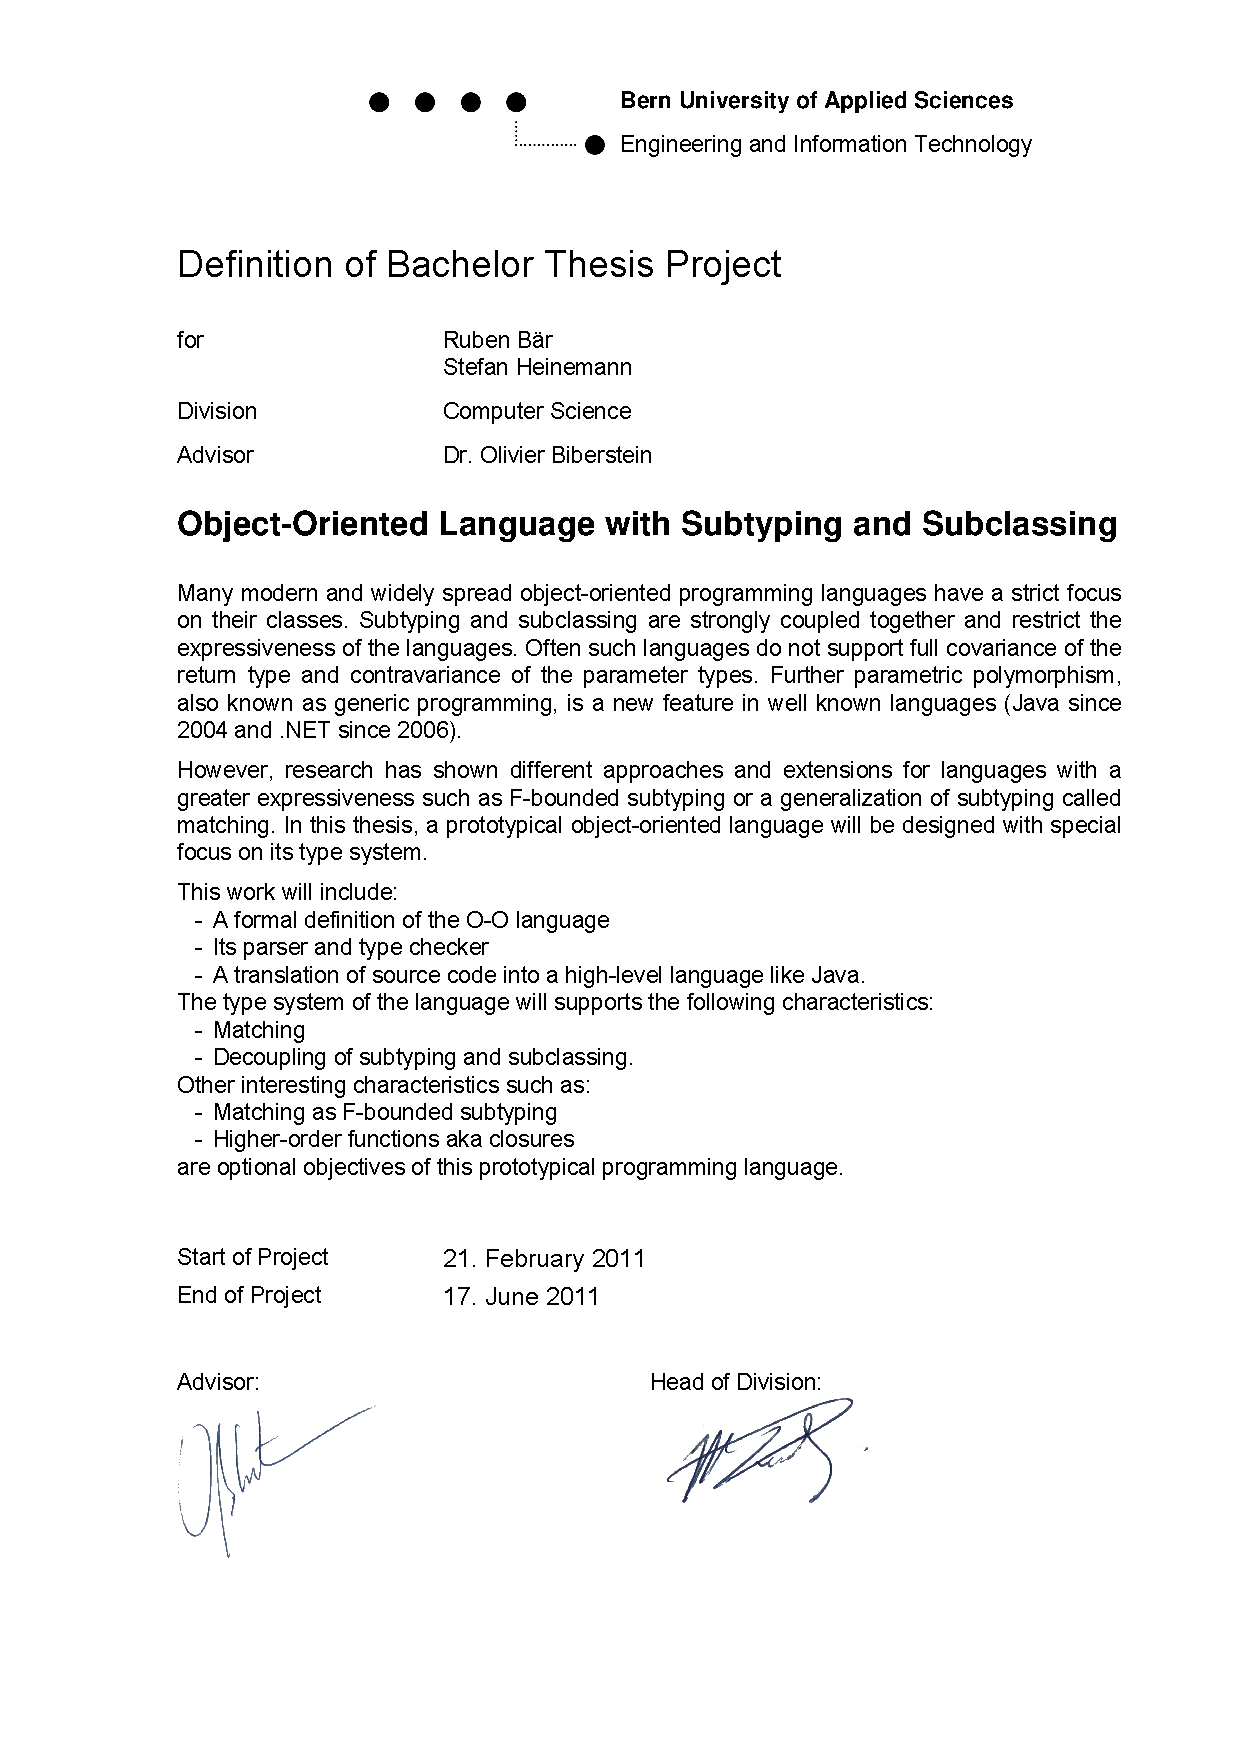
\includegraphics[height=\textheight,keepaspectratio=true]{../proposal}
\setlength\fboxsep{0pt}
\setlength\fboxrule{0.5pt}
\fbox{
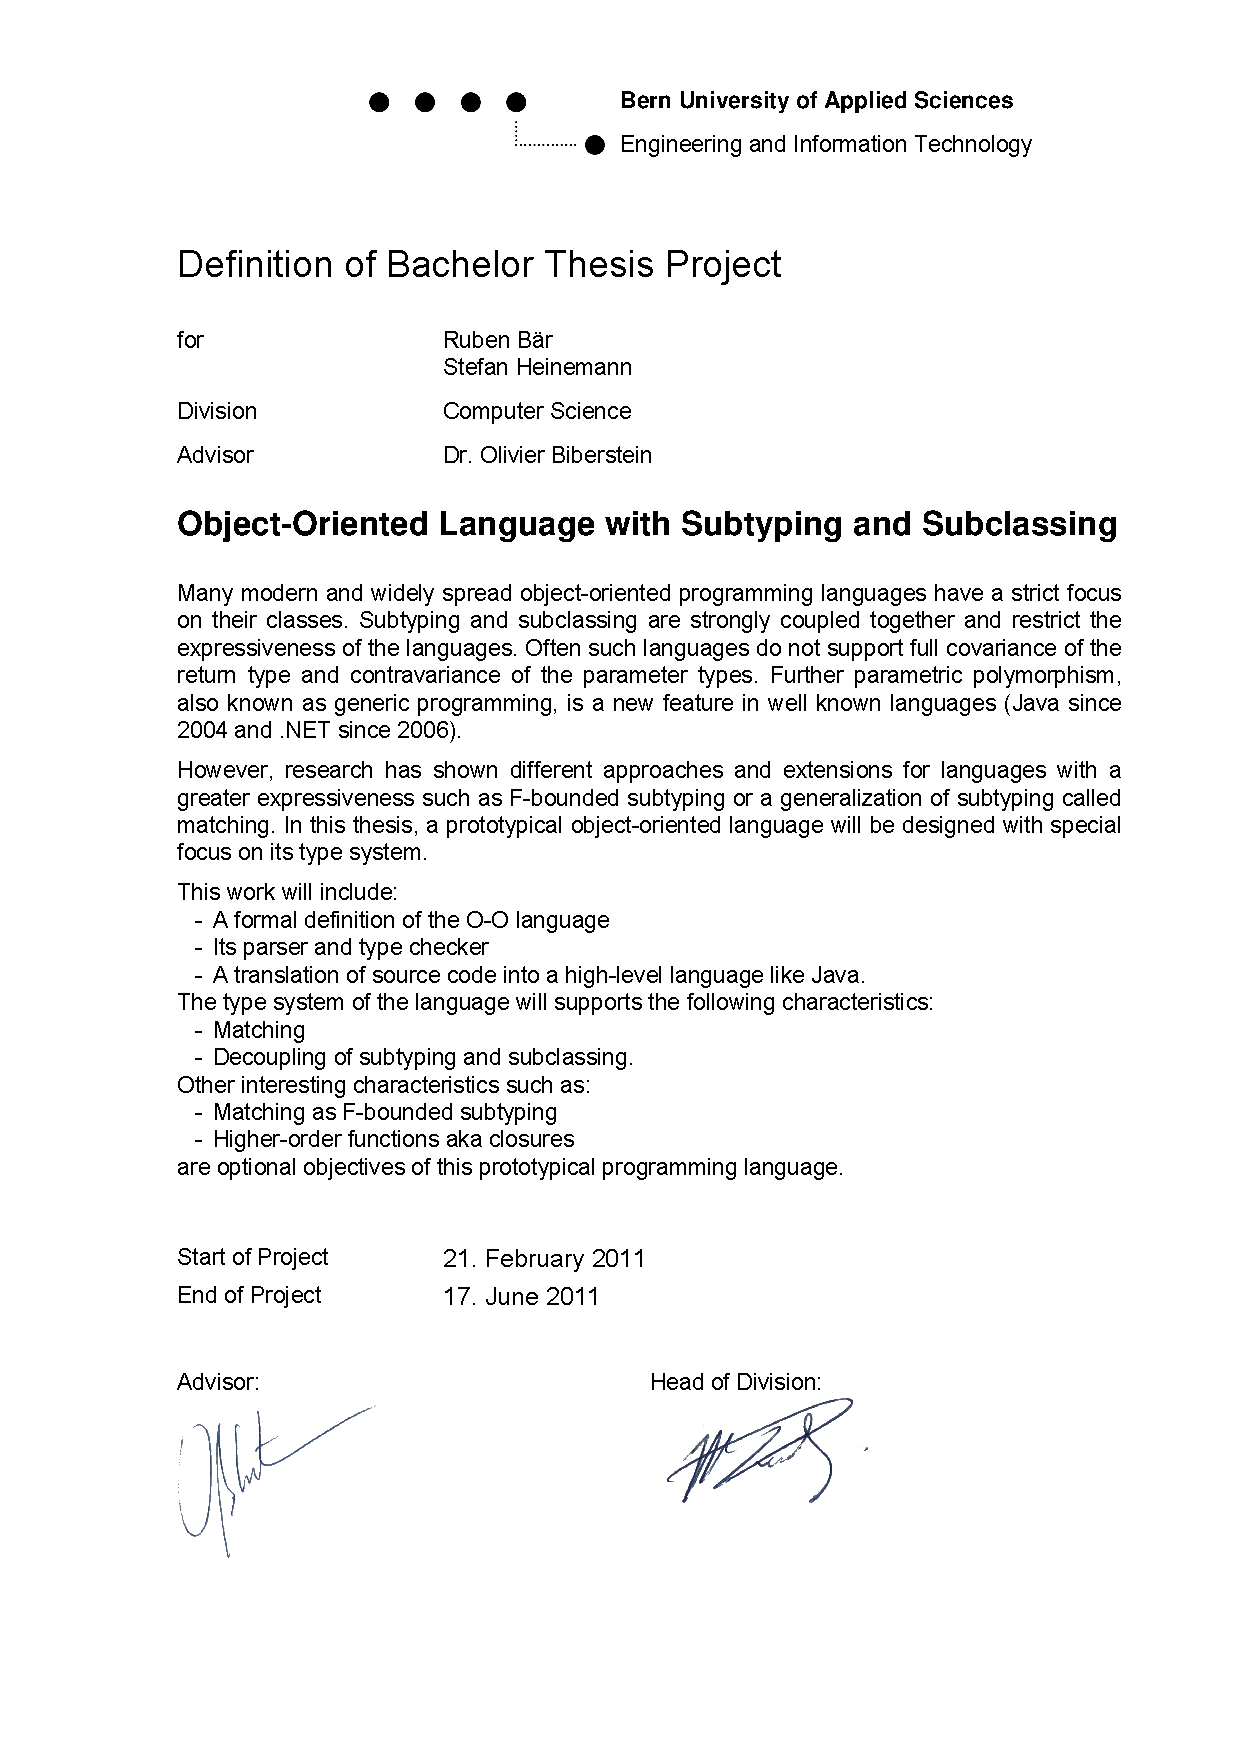
\includegraphics[scale=0.58]{../proposal}
}
\end{figure}

% estimated pages: 


\addcontentsline{toc}{chapter}{Bibliography}
\bibliography{bib/ooplss,bib/simons}

\end{empfile}
\end{document}

  \begin{frame}[t]{Zeitplan}
	\scalebox{0.7}{
	\begin{gantt}[xunitlength=0.7cm]{12}{16}
		\begin{ganttitle}
			\numtitle{1}{1}{16}{1}
		\end{ganttitle}
		\ganttbar{Kick-Off}{0}{2}
		\ganttbarcon{Documentation Part I / II}{2}{3}
		\ganttbar{Grammar / Lexer}{3}{2}
		\ganttbarcon{Types}{5}{2}
		\ganttbar{Parser}{5}{3} % Con
		\ganttbar{Tree Walking}{8}{1}
		\ganttbarcon{Symbol Table Construction}{9}{1}
		\ganttbar{Type Checker}{9}{6} % Con
		\ganttbar{Code Translation Definition}{6}{2}
		\ganttbarcon{Code Translation}{11}{5}
		\ganttbar{Documentation}{0}{16}

		\ganttcon{5}{3}{5}{5}
		\ganttcon{8}{5}{8}{6}
		\ganttcon{8}{5}{8}{6}
		\ganttcon{9}{6}{9}{8}
	\end{gantt}}
\end{frame}

  \begin{frame}[t]{Dokumentation}
  \begin{bigitemize}[<+->]{3mm}
<<<<<<< HEAD
<<<<<<< HEAD
		\item Probleme aufzeigen
=======
		\item Probleme aufzeiten
>>>>>>> Meeting: Slides written
=======
		\item Probleme aufzeigen
>>>>>>> Meeting: writting corrections
		\item Lösungsvarianten anbieten
		\item Spezifikation
		\item Implementierung
		\begin{itemize}
			\item Code Dokumentation
<<<<<<< HEAD
<<<<<<< HEAD
			\item Spezielles und Generelles in Dokumentation
=======
			\item Spezielles und generelles in Dokumentation
>>>>>>> Meeting: Slides written
=======
			\item Spezielles und Generelles in Dokumentation
>>>>>>> Meeting: writting corrections
		\end{itemize}
	\end{bigitemize}
\end{frame}

  \begin{frame}[t]{Fragen?}
\end{frame}

  \begin{frame}[t]{Varia}
  \begin{bigitemize}{3mm}
    \item Nächstes Meeting

    \item Datum für Verteidigung
  \end{bigitemize}
\end{frame}

<<<<<<< HEAD
=======
>>>>>>> Meeting: Presentation for the first expert meeting
=======
>>>>>>> Meeting: Gantt
\end{document}
